% lecture2.tex -- GENERATED by build_L2.py from L2_numbers.json; do not edit by hand.
\documentclass[10pt,aspectratio=169,t]{beamer}
% =============================================================================
% nn_preamble.tex -- shared Beamer preamble of Neural Networks and Deep Learning (NN)
% Used by every lecture: lectures/Lk/lecturek.tex does
%   \documentclass[10pt,aspectratio=169,t]{beamer}
%   % =============================================================================
% nn_preamble.tex -- shared Beamer preamble of Neural Networks and Deep Learning (NN)
% Used by every lecture: lectures/Lk/lecturek.tex does
%   \documentclass[10pt,aspectratio=169,t]{beamer}
%   % =============================================================================
% nn_preamble.tex -- shared Beamer preamble of Neural Networks and Deep Learning (NN)
% Used by every lecture: lectures/Lk/lecturek.tex does
%   \documentclass[10pt,aspectratio=169,t]{beamer}
%   \input{../common/nn_preamble}
%   \nnlecture{k}{Lecture title}
% Logos live in lectures/common/logos/, charts in lectures/Lk/charts/.
% Do NOT add \hfuzz / \vfuzz / \hbadness here: overfull boxes must be fixed, not hidden.
% =============================================================================

\usetheme{default}
\setbeamersize{text margin left=7mm, text margin right=7mm}

% ---------------------------------------------------------------- packages
\usepackage[utf8]{inputenc}
\usepackage[T1]{fontenc}
\usepackage{lmodern}
\usepackage{amsmath, amssymb}
\usepackage{mathtools}
\usepackage{bm}
\usepackage{tikz}
\usetikzlibrary{arrows.meta, positioning, calc, shapes.misc}
\usepackage{booktabs}
\usepackage{array}
\usepackage{graphicx}
\usepackage{colortbl}
\usepackage{xcolor}
\usepackage{multicol}
\hypersetup{colorlinks=true, linkcolor=MainBlue, urlcolor=MainBlue, citecolor=MainBlue}
\graphicspath{{../common/logos/}}   % charts are included with their language folder: charts/en/, charts/ro/

% ---------------------------------------------------------------- colours
\definecolor{MainBlue}{RGB}{26, 58, 110}
\definecolor{IDAred}{RGB}{205, 0, 0}
\definecolor{DarkGray}{RGB}{51, 51, 51}
\definecolor{FooterGray}{RGB}{100, 100, 100}
\definecolor{BlockGray}{RGB}{236, 238, 242}
\definecolor{KeynoteGray}{RGB}{218, 218, 218}
\definecolor{Crimson}{RGB}{190, 40, 50}
\definecolor{Forest}{RGB}{30, 110, 50}
\definecolor{Bitter}{RGB}{214, 150, 20}
% chart palette (same hex values and order as lectures/common/nn_plot.py SERIES)
\definecolor{Ser1}{HTML}{2A78D6}
\definecolor{Ser2}{HTML}{EB6834}
\definecolor{Ser3}{HTML}{1BAF7A}
\definecolor{Ser4}{HTML}{EDA100}
\definecolor{Ser5}{HTML}{E87BA4}
\definecolor{Ser6}{HTML}{008300}
\definecolor{Ser7}{HTML}{6250D6}
\definecolor{Ser8}{HTML}{E34948}

\setbeamertemplate{background}{%
  \begin{tikzpicture}[remember picture, overlay]
    \shade[shading=axis, shading angle=315, top color=white, bottom color=KeynoteGray]
      (current page.south west) rectangle (current page.north east);
  \end{tikzpicture}}
\setbeamercolor{background canvas}{bg=}
\setbeamercolor{structure}{fg=MainBlue}
\setbeamercolor{normal text}{fg=DarkGray}
\setbeamercolor{title}{fg=IDAred}
\setbeamercolor{frametitle}{fg=IDAred, bg=}
\setbeamercolor{block title}{bg=MainBlue, fg=white}
\setbeamercolor{block body}{bg=BlockGray, fg=DarkGray}
\setbeamercolor{block title alerted}{bg=Crimson, fg=white}
\setbeamercolor{block body alerted}{bg=Crimson!7, fg=DarkGray}
\setbeamercolor{block title example}{bg=Forest, fg=white}
\setbeamercolor{block body example}{bg=Forest!7, fg=DarkGray}
\setbeamercolor{item}{fg=MainBlue}
\setbeamerfont{frametitle}{size=\large, series=\bfseries}
\setbeamerfont{block title}{size=\small, series=\bfseries}
\setbeamertemplate{blocks}[rounded][shadow=false]
\setbeamertemplate{itemize item}{\color{MainBlue}$\boxdot$}
\setbeamertemplate{itemize subitem}{\color{MainBlue}\scriptsize$\blacktriangleright$}
% compact two-level lists: level 1 = main point, level 2 = details (no text outside bullets)
\setbeamerfont{itemize/enumerate subbody}{size=\footnotesize}
\setlength{\leftmargini}{1.1em}
\setlength{\leftmarginii}{1.1em}
\setbeamertemplate{itemize/enumerate body begin}{\setlength{\topsep}{0pt}\setlength{\partopsep}{0pt}\setlength{\parskip}{0pt}}
\setbeamertemplate{itemize/enumerate subbody begin}{\setlength{\topsep}{0pt}\setlength{\partopsep}{0pt}\setlength{\itemsep}{0pt}\vspace{-0.4ex}}

\setbeamertemplate{enumerate item}{\color{MainBlue}\insertenumlabel.}
\setlength{\leftmargini}{1.3em}
\setlength{\leftmarginii}{1.2em}
\setbeamertemplate{navigation symbols}{}
\setbeamertemplate{section in toc}{\color{MainBlue}$\blacktriangleright$~\inserttocsection}
\setbeamertemplate{caption}{\raggedright\insertcaption\par}
% frame subtitle = precise citation line under the claim title (Weron style)
\setbeamerfont{framesubtitle}{size=\footnotesize}
\setbeamercolor{framesubtitle}{fg=FooterGray}
% outline that reappears at every section with the current section highlighted
\setbeamertemplate{section in toc shaded}[default][35]
\setbeamertemplate{subsection in toc shaded}[default][35]
\setbeamertemplate{subsection in toc}{\leavevmode\leftskip=2.2em\color{DarkGray}\small\inserttocsubsection\par}
\AtBeginSection[]{{\begin{frame}{\txtoutline}\vspace{2mm}\small
  \tableofcontents[currentsection,hideothersubsections]\end{frame}}}

% ---------------------------------------------------------------- head and foot
\setbeamertemplate{headline}{%
  \vskip10pt%
  \hbox to \paperwidth{\hskip0.5cm%
    {\small\color{FooterGray}\renewcommand{\hyperlink}[2]{##2}\insertsectionhead}%
    \hfill\textcolor{FooterGray}{\small\insertframenumber}\hskip0.5cm}%
  \vskip4pt{\color{FooterGray}\hrule height 0.4pt}}
% footer as in the other courses (MFM, SFM): course name on the left, small sparkline on the right
\setbeamertemplate{footline}{%
  {\color{FooterGray}\hrule height 0.4pt}\vskip4pt%
  \hbox to \paperwidth{\hskip0.5cm%
    \textcolor{FooterGray}{\small\txtcourse}%
    \hfill\raisebox{-0.1em}{\begin{tikzpicture}[x=0.08em, y=0.08em, line width=0.4pt]
      \draw[FooterGray] (0,3) -- (1,4) -- (2,3.5) -- (3,5) -- (4,4) -- (5,6) -- (6,5.5) -- (7,4) -- (8,5) -- (9,7) -- (10,6) -- (11,5) -- (12,6.5) -- (13,8) -- (14,7) -- (15,6) -- (16,7.5) -- (17,9) -- (18,8) -- (19,7) -- (20,8.5) -- (21,10) -- (22,9) -- (23,8) -- (24,9.5);
    \end{tikzpicture}}\hskip0.5cm}%
  \vskip6pt}

% ---------------------------------------------------------------- title page
\defbeamertemplate*{title page}{nn}[1][]{%
  \vspace{0.15cm}
  \begin{center}
    \href{https://www.ase.ro}{
\includegraphics[height=0.9cm]{ase_logo.png}}\hspace{0.3cm}%
    \href{https://ipe.ro/new}{
\includegraphics[height=0.9cm]{acad_logo.png}}\hspace{0.3cm}%
    \href{https://theida.net}{
\includegraphics[height=0.9cm]{ida_logo.png}}\hspace{0.3cm}%
    \href{https://blockchain-research-center.com}{
\includegraphics[height=0.9cm]{brc_logo.png}}\hspace{0.3cm}%
    \href{https://www.ai4efin.ase.ro}{
\includegraphics[height=0.9cm]{ai4efin_logo.png}}\hspace{0.3cm}%
    \href{https://www.digital-finance-msca.com}{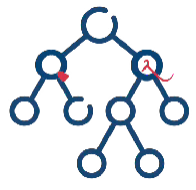
\includegraphics[height=0.9cm]{msca_logo.png}}%
  \end{center}
  \vspace{0.45cm}
  \begin{center}
    \begin{minipage}{0.1\textwidth}\centering
      \href{https://quantlet.com}{
\includegraphics[height=0.9cm]{ql_logo.png}}\end{minipage}%
    \begin{minipage}{0.78\textwidth}\centering
      {\Large\bfseries\usebeamercolor[fg]{title}\inserttitle}\par\vspace{0.25cm}
      {\large\usebeamercolor[fg]{title}\insertsubtitle}\end{minipage}%
    \begin{minipage}{0.1\textwidth}\centering
      \href{https://quantinar.com}{
\includegraphics[height=0.9cm]{qr_logo.png}}\end{minipage}
  \end{center}
  \vfill
  \hspace{0.4cm}{\bfseries\insertauthor}\par\vspace{0.12cm}
  \hspace{0.4cm}\begin{minipage}[t]{0.92\textwidth}\raggedright\footnotesize\insertinstitute\end{minipage}
  \par\vspace{0.4cm}}

% ---------------------------------------------------------------- lecture metadata
\newcommand{\nnshort}{}
\newcommand{\nnnb}{notebooks}
\newcommand{\nnrepo}{https://github.com/danpele/NEURAL_BIZ/tree/main}
% language-dependent labels (English default; \nnromanian switches to Romanian, call it before \nnlecture)
\newcommand{\txtcourse}{Neural Networks and Deep Learning}
\newcommand{\txtlecture}{Lecture}
\newcommand{\txtoutline}{Outline}
\newcommand{\txtintuition}{In one sentence:}
\newcommand{\txtjob}{In practice:}
\newcommand{\txttry}{Experiment yourself:}
\newcommand{\txtwhere}{where}
\newcommand{\txtsim}{SIMULATED DATA (teaching illustration)}
\newcommand{\txtnbsuffix}{}
\newcommand{\txtinstitute}{Bucharest University of Economic Studies (ASE), Department of Statistics and Econometrics\\
    Romanian Academy, Institute for Economic Forecasting (IPE)\\
    IDA Institute Digital Assets \textbullet\ AI4EFin \textbullet\ MSCA Digital Finance}
\newcommand{\nnromanian}{%
  \renewcommand{\txtcourse}{Rețele neuronale și deep learning}%
  \renewcommand{\txtlecture}{Cursul}%
  \renewcommand{\txtoutline}{Cuprins}%
  \renewcommand{\txtintuition}{Pe scurt:}%
  \renewcommand{\txtjob}{În practică:}%
  \renewcommand{\txttry}{Exercițiu practic:}%
  \renewcommand{\txtwhere}{unde}%
  \renewcommand{\txtsim}{DATE SIMULATE (doar pentru ilustrare)}%
  \renewcommand{\txtnbsuffix}{\string_ro}%
  \renewcommand{\txtinstitute}{Academia de Studii Economice din București (ASE), Departamentul de Statistică și Econometrie\\
    Academia Română, Institutul de Prognoză Economică (IPE)\\
    IDA Institute Digital Assets \textbullet\ AI4EFin \textbullet\ MSCA Digital Finance}}
\newcommand{\nnlecture}[2]{%
  \renewcommand{\nnshort}{\txtlecture\ #1}%
  \renewcommand{\nnnb}{notebooks/L#1\string_notebook\txtnbsuffix.ipynb}%
  \title[NN]{\txtcourse}%
  \subtitle{\txtlecture\ #1: #2}%
  \author{Prof.\ dr.\ Daniel Traian PELE}%
  \institute{\txtinstitute}%
  \date{}}

% ---------------------------------------------------------------- teaching blocks (one message per frame)
% \intuition{one plain sentence}  ->  formula with every symbol defined  ->  real-data example  ->  \manager{one line}
\newcommand{\intuition}[1]{\begin{itemize}\item {\color{MainBlue}\textbf{\txtintuition}}~#1\end{itemize}\vspace{0.6mm}}
\newcommand{\manager}[1]{\colorbox{Forest!10}{\parbox{\dimexpr\linewidth-2\fboxsep\relax}{\footnotesize
  \begin{itemize}\setlength{\itemsep}{0pt}\item \textbf{\color{Forest}\txtjob}~#1\end{itemize}}}}
% Experiment yourself: pointer to the matching notebook section
\newcommand{\tryit}[1]{{\scriptsize\href{\nnrepo/\nnnb}{%
  \raisebox{-0.15em}{
\includegraphics[height=0.85em]{ql_logo.png}}\,\textbf{\txttry}~\color{MainBlue}#1}}}
% bottom row: manager line (left) + experiment pointer (right), pinned to the bottom of the frame
\newcommand{\bottomrow}[2]{\par\vfill\noindent\begin{minipage}[b]{0.72\linewidth}#1\end{minipage}\hfill
  \begin{minipage}[b]{0.26\linewidth}\raggedleft #2\end{minipage}\par\vspace{0.5mm}}
\newcommand{\where}[1]{{\footnotesize\textbf{\txtwhere}~#1\par}}

% ---------------------------------------------------------------- helpers
% chart source line under a figure: \chartsource{Source ...; period ...}
\newcommand{\chartsource}[1]{\par\vspace{1pt}{\scriptsize\color{FooterGray}#1\par}}
% link to code: \quantlet{label}{path inside the repo}
\newcommand{\quantlet}[2]{\par\vspace{1pt}\hfill\href{\nnrepo/#2}{%
  \raisebox{-0.15em}{
\includegraphics[height=0.75em]{ql_logo.png}}\textcolor{MainBlue}{\scriptsize\ #1}}}
% inline Quantlet link for the bottom-right corner of a frame: \qlink{label}{path inside the repo}
\newcommand{\qlink}[2]{{\scriptsize\href{\nnrepo/#2}{\raisebox{-0.15em}{
\includegraphics[height=0.85em]{ql_logo.png}}\,\textcolor{MainBlue}{#1}}}}
\newcommand{\simlabel}{\colorbox{Crimson!12}{\scriptsize\bfseries\color{Crimson}\txtsim}}
\newcommand{\E}{\mathbb{E}}
\newcommand{\Var}{\operatorname{Var}}
\newcommand{\Cov}{\operatorname{Cov}}
\newcommand{\Corr}{\operatorname{Corr}}
\newcommand{\asinh}{\operatorname{asinh}}
\newcommand{\iid}{\overset{\text{i.i.d.}}{\sim}}
\newcommand{\EUR}{EUR}
% deep-learning notation (Bishop & Bishop, 2024): vectors bold lower case, matrices bold upper case
\newcommand{\R}{\mathbb{R}}
\newcommand{\vx}{\mathbf{x}}
\newcommand{\vy}{\mathbf{y}}
\newcommand{\vz}{\mathbf{z}}
\newcommand{\vh}{\mathbf{h}}
\newcommand{\vw}{\mathbf{w}}
\newcommand{\vb}{\mathbf{b}}
\newcommand{\mW}{\mathbf{W}}
\newcommand{\mX}{\mathbf{X}}
\newcommand{\btheta}{\boldsymbol{\theta}}
\newcommand{\loss}{\mathcal{L}}
\newcommand{\dataset}{\mathcal{D}}
\DeclareMathOperator*{\argmin}{arg\,min}
\DeclareMathOperator*{\argmax}{arg\,max}
\DeclareMathOperator{\softmax}{softmax}
\DeclareMathOperator{\ReLU}{ReLU}
\DeclareMathOperator{\sigm}{\sigma}

%   \nnlecture{k}{Lecture title}
% Logos live in lectures/common/logos/, charts in lectures/Lk/charts/.
% Do NOT add \hfuzz / \vfuzz / \hbadness here: overfull boxes must be fixed, not hidden.
% =============================================================================

\usetheme{default}
\setbeamersize{text margin left=7mm, text margin right=7mm}

% ---------------------------------------------------------------- packages
\usepackage[utf8]{inputenc}
\usepackage[T1]{fontenc}
\usepackage{lmodern}
\usepackage{amsmath, amssymb}
\usepackage{mathtools}
\usepackage{bm}
\usepackage{tikz}
\usetikzlibrary{arrows.meta, positioning, calc, shapes.misc}
\usepackage{booktabs}
\usepackage{array}
\usepackage{graphicx}
\usepackage{colortbl}
\usepackage{xcolor}
\usepackage{multicol}
\hypersetup{colorlinks=true, linkcolor=MainBlue, urlcolor=MainBlue, citecolor=MainBlue}
\graphicspath{{../common/logos/}}   % charts are included with their language folder: charts/en/, charts/ro/

% ---------------------------------------------------------------- colours
\definecolor{MainBlue}{RGB}{26, 58, 110}
\definecolor{IDAred}{RGB}{205, 0, 0}
\definecolor{DarkGray}{RGB}{51, 51, 51}
\definecolor{FooterGray}{RGB}{100, 100, 100}
\definecolor{BlockGray}{RGB}{236, 238, 242}
\definecolor{KeynoteGray}{RGB}{218, 218, 218}
\definecolor{Crimson}{RGB}{190, 40, 50}
\definecolor{Forest}{RGB}{30, 110, 50}
\definecolor{Bitter}{RGB}{214, 150, 20}
% chart palette (same hex values and order as lectures/common/nn_plot.py SERIES)
\definecolor{Ser1}{HTML}{2A78D6}
\definecolor{Ser2}{HTML}{EB6834}
\definecolor{Ser3}{HTML}{1BAF7A}
\definecolor{Ser4}{HTML}{EDA100}
\definecolor{Ser5}{HTML}{E87BA4}
\definecolor{Ser6}{HTML}{008300}
\definecolor{Ser7}{HTML}{6250D6}
\definecolor{Ser8}{HTML}{E34948}

\setbeamertemplate{background}{%
  \begin{tikzpicture}[remember picture, overlay]
    \shade[shading=axis, shading angle=315, top color=white, bottom color=KeynoteGray]
      (current page.south west) rectangle (current page.north east);
  \end{tikzpicture}}
\setbeamercolor{background canvas}{bg=}
\setbeamercolor{structure}{fg=MainBlue}
\setbeamercolor{normal text}{fg=DarkGray}
\setbeamercolor{title}{fg=IDAred}
\setbeamercolor{frametitle}{fg=IDAred, bg=}
\setbeamercolor{block title}{bg=MainBlue, fg=white}
\setbeamercolor{block body}{bg=BlockGray, fg=DarkGray}
\setbeamercolor{block title alerted}{bg=Crimson, fg=white}
\setbeamercolor{block body alerted}{bg=Crimson!7, fg=DarkGray}
\setbeamercolor{block title example}{bg=Forest, fg=white}
\setbeamercolor{block body example}{bg=Forest!7, fg=DarkGray}
\setbeamercolor{item}{fg=MainBlue}
\setbeamerfont{frametitle}{size=\large, series=\bfseries}
\setbeamerfont{block title}{size=\small, series=\bfseries}
\setbeamertemplate{blocks}[rounded][shadow=false]
\setbeamertemplate{itemize item}{\color{MainBlue}$\boxdot$}
\setbeamertemplate{itemize subitem}{\color{MainBlue}\scriptsize$\blacktriangleright$}
% compact two-level lists: level 1 = main point, level 2 = details (no text outside bullets)
\setbeamerfont{itemize/enumerate subbody}{size=\footnotesize}
\setlength{\leftmargini}{1.1em}
\setlength{\leftmarginii}{1.1em}
\setbeamertemplate{itemize/enumerate body begin}{\setlength{\topsep}{0pt}\setlength{\partopsep}{0pt}\setlength{\parskip}{0pt}}
\setbeamertemplate{itemize/enumerate subbody begin}{\setlength{\topsep}{0pt}\setlength{\partopsep}{0pt}\setlength{\itemsep}{0pt}\vspace{-0.4ex}}

\setbeamertemplate{enumerate item}{\color{MainBlue}\insertenumlabel.}
\setlength{\leftmargini}{1.3em}
\setlength{\leftmarginii}{1.2em}
\setbeamertemplate{navigation symbols}{}
\setbeamertemplate{section in toc}{\color{MainBlue}$\blacktriangleright$~\inserttocsection}
\setbeamertemplate{caption}{\raggedright\insertcaption\par}
% frame subtitle = precise citation line under the claim title (Weron style)
\setbeamerfont{framesubtitle}{size=\footnotesize}
\setbeamercolor{framesubtitle}{fg=FooterGray}
% outline that reappears at every section with the current section highlighted
\setbeamertemplate{section in toc shaded}[default][35]
\setbeamertemplate{subsection in toc shaded}[default][35]
\setbeamertemplate{subsection in toc}{\leavevmode\leftskip=2.2em\color{DarkGray}\small\inserttocsubsection\par}
\AtBeginSection[]{{\begin{frame}{\txtoutline}\vspace{2mm}\small
  \tableofcontents[currentsection,hideothersubsections]\end{frame}}}

% ---------------------------------------------------------------- head and foot
\setbeamertemplate{headline}{%
  \vskip10pt%
  \hbox to \paperwidth{\hskip0.5cm%
    {\small\color{FooterGray}\renewcommand{\hyperlink}[2]{##2}\insertsectionhead}%
    \hfill\textcolor{FooterGray}{\small\insertframenumber}\hskip0.5cm}%
  \vskip4pt{\color{FooterGray}\hrule height 0.4pt}}
% footer as in the other courses (MFM, SFM): course name on the left, small sparkline on the right
\setbeamertemplate{footline}{%
  {\color{FooterGray}\hrule height 0.4pt}\vskip4pt%
  \hbox to \paperwidth{\hskip0.5cm%
    \textcolor{FooterGray}{\small\txtcourse}%
    \hfill\raisebox{-0.1em}{\begin{tikzpicture}[x=0.08em, y=0.08em, line width=0.4pt]
      \draw[FooterGray] (0,3) -- (1,4) -- (2,3.5) -- (3,5) -- (4,4) -- (5,6) -- (6,5.5) -- (7,4) -- (8,5) -- (9,7) -- (10,6) -- (11,5) -- (12,6.5) -- (13,8) -- (14,7) -- (15,6) -- (16,7.5) -- (17,9) -- (18,8) -- (19,7) -- (20,8.5) -- (21,10) -- (22,9) -- (23,8) -- (24,9.5);
    \end{tikzpicture}}\hskip0.5cm}%
  \vskip6pt}

% ---------------------------------------------------------------- title page
\defbeamertemplate*{title page}{nn}[1][]{%
  \vspace{0.15cm}
  \begin{center}
    \href{https://www.ase.ro}{
\includegraphics[height=0.9cm]{ase_logo.png}}\hspace{0.3cm}%
    \href{https://ipe.ro/new}{
\includegraphics[height=0.9cm]{acad_logo.png}}\hspace{0.3cm}%
    \href{https://theida.net}{
\includegraphics[height=0.9cm]{ida_logo.png}}\hspace{0.3cm}%
    \href{https://blockchain-research-center.com}{
\includegraphics[height=0.9cm]{brc_logo.png}}\hspace{0.3cm}%
    \href{https://www.ai4efin.ase.ro}{
\includegraphics[height=0.9cm]{ai4efin_logo.png}}\hspace{0.3cm}%
    \href{https://www.digital-finance-msca.com}{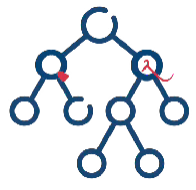
\includegraphics[height=0.9cm]{msca_logo.png}}%
  \end{center}
  \vspace{0.45cm}
  \begin{center}
    \begin{minipage}{0.1\textwidth}\centering
      \href{https://quantlet.com}{
\includegraphics[height=0.9cm]{ql_logo.png}}\end{minipage}%
    \begin{minipage}{0.78\textwidth}\centering
      {\Large\bfseries\usebeamercolor[fg]{title}\inserttitle}\par\vspace{0.25cm}
      {\large\usebeamercolor[fg]{title}\insertsubtitle}\end{minipage}%
    \begin{minipage}{0.1\textwidth}\centering
      \href{https://quantinar.com}{
\includegraphics[height=0.9cm]{qr_logo.png}}\end{minipage}
  \end{center}
  \vfill
  \hspace{0.4cm}{\bfseries\insertauthor}\par\vspace{0.12cm}
  \hspace{0.4cm}\begin{minipage}[t]{0.92\textwidth}\raggedright\footnotesize\insertinstitute\end{minipage}
  \par\vspace{0.4cm}}

% ---------------------------------------------------------------- lecture metadata
\newcommand{\nnshort}{}
\newcommand{\nnnb}{notebooks}
\newcommand{\nnrepo}{https://github.com/danpele/NEURAL_BIZ/tree/main}
% language-dependent labels (English default; \nnromanian switches to Romanian, call it before \nnlecture)
\newcommand{\txtcourse}{Neural Networks and Deep Learning}
\newcommand{\txtlecture}{Lecture}
\newcommand{\txtoutline}{Outline}
\newcommand{\txtintuition}{In one sentence:}
\newcommand{\txtjob}{In practice:}
\newcommand{\txttry}{Experiment yourself:}
\newcommand{\txtwhere}{where}
\newcommand{\txtsim}{SIMULATED DATA (teaching illustration)}
\newcommand{\txtnbsuffix}{}
\newcommand{\txtinstitute}{Bucharest University of Economic Studies (ASE), Department of Statistics and Econometrics\\
    Romanian Academy, Institute for Economic Forecasting (IPE)\\
    IDA Institute Digital Assets \textbullet\ AI4EFin \textbullet\ MSCA Digital Finance}
\newcommand{\nnromanian}{%
  \renewcommand{\txtcourse}{Rețele neuronale și deep learning}%
  \renewcommand{\txtlecture}{Cursul}%
  \renewcommand{\txtoutline}{Cuprins}%
  \renewcommand{\txtintuition}{Pe scurt:}%
  \renewcommand{\txtjob}{În practică:}%
  \renewcommand{\txttry}{Exercițiu practic:}%
  \renewcommand{\txtwhere}{unde}%
  \renewcommand{\txtsim}{DATE SIMULATE (doar pentru ilustrare)}%
  \renewcommand{\txtnbsuffix}{\string_ro}%
  \renewcommand{\txtinstitute}{Academia de Studii Economice din București (ASE), Departamentul de Statistică și Econometrie\\
    Academia Română, Institutul de Prognoză Economică (IPE)\\
    IDA Institute Digital Assets \textbullet\ AI4EFin \textbullet\ MSCA Digital Finance}}
\newcommand{\nnlecture}[2]{%
  \renewcommand{\nnshort}{\txtlecture\ #1}%
  \renewcommand{\nnnb}{notebooks/L#1\string_notebook\txtnbsuffix.ipynb}%
  \title[NN]{\txtcourse}%
  \subtitle{\txtlecture\ #1: #2}%
  \author{Prof.\ dr.\ Daniel Traian PELE}%
  \institute{\txtinstitute}%
  \date{}}

% ---------------------------------------------------------------- teaching blocks (one message per frame)
% \intuition{one plain sentence}  ->  formula with every symbol defined  ->  real-data example  ->  \manager{one line}
\newcommand{\intuition}[1]{\begin{itemize}\item {\color{MainBlue}\textbf{\txtintuition}}~#1\end{itemize}\vspace{0.6mm}}
\newcommand{\manager}[1]{\colorbox{Forest!10}{\parbox{\dimexpr\linewidth-2\fboxsep\relax}{\footnotesize
  \begin{itemize}\setlength{\itemsep}{0pt}\item \textbf{\color{Forest}\txtjob}~#1\end{itemize}}}}
% Experiment yourself: pointer to the matching notebook section
\newcommand{\tryit}[1]{{\scriptsize\href{\nnrepo/\nnnb}{%
  \raisebox{-0.15em}{
\includegraphics[height=0.85em]{ql_logo.png}}\,\textbf{\txttry}~\color{MainBlue}#1}}}
% bottom row: manager line (left) + experiment pointer (right), pinned to the bottom of the frame
\newcommand{\bottomrow}[2]{\par\vfill\noindent\begin{minipage}[b]{0.72\linewidth}#1\end{minipage}\hfill
  \begin{minipage}[b]{0.26\linewidth}\raggedleft #2\end{minipage}\par\vspace{0.5mm}}
\newcommand{\where}[1]{{\footnotesize\textbf{\txtwhere}~#1\par}}

% ---------------------------------------------------------------- helpers
% chart source line under a figure: \chartsource{Source ...; period ...}
\newcommand{\chartsource}[1]{\par\vspace{1pt}{\scriptsize\color{FooterGray}#1\par}}
% link to code: \quantlet{label}{path inside the repo}
\newcommand{\quantlet}[2]{\par\vspace{1pt}\hfill\href{\nnrepo/#2}{%
  \raisebox{-0.15em}{
\includegraphics[height=0.75em]{ql_logo.png}}\textcolor{MainBlue}{\scriptsize\ #1}}}
% inline Quantlet link for the bottom-right corner of a frame: \qlink{label}{path inside the repo}
\newcommand{\qlink}[2]{{\scriptsize\href{\nnrepo/#2}{\raisebox{-0.15em}{
\includegraphics[height=0.85em]{ql_logo.png}}\,\textcolor{MainBlue}{#1}}}}
\newcommand{\simlabel}{\colorbox{Crimson!12}{\scriptsize\bfseries\color{Crimson}\txtsim}}
\newcommand{\E}{\mathbb{E}}
\newcommand{\Var}{\operatorname{Var}}
\newcommand{\Cov}{\operatorname{Cov}}
\newcommand{\Corr}{\operatorname{Corr}}
\newcommand{\asinh}{\operatorname{asinh}}
\newcommand{\iid}{\overset{\text{i.i.d.}}{\sim}}
\newcommand{\EUR}{EUR}
% deep-learning notation (Bishop & Bishop, 2024): vectors bold lower case, matrices bold upper case
\newcommand{\R}{\mathbb{R}}
\newcommand{\vx}{\mathbf{x}}
\newcommand{\vy}{\mathbf{y}}
\newcommand{\vz}{\mathbf{z}}
\newcommand{\vh}{\mathbf{h}}
\newcommand{\vw}{\mathbf{w}}
\newcommand{\vb}{\mathbf{b}}
\newcommand{\mW}{\mathbf{W}}
\newcommand{\mX}{\mathbf{X}}
\newcommand{\btheta}{\boldsymbol{\theta}}
\newcommand{\loss}{\mathcal{L}}
\newcommand{\dataset}{\mathcal{D}}
\DeclareMathOperator*{\argmin}{arg\,min}
\DeclareMathOperator*{\argmax}{arg\,max}
\DeclareMathOperator{\softmax}{softmax}
\DeclareMathOperator{\ReLU}{ReLU}
\DeclareMathOperator{\sigm}{\sigma}

%   \nnlecture{k}{Lecture title}
% Logos live in lectures/common/logos/, charts in lectures/Lk/charts/.
% Do NOT add \hfuzz / \vfuzz / \hbadness here: overfull boxes must be fixed, not hidden.
% =============================================================================

\usetheme{default}
\setbeamersize{text margin left=7mm, text margin right=7mm}

% ---------------------------------------------------------------- packages
\usepackage[utf8]{inputenc}
\usepackage[T1]{fontenc}
\usepackage{lmodern}
\usepackage{amsmath, amssymb}
\usepackage{mathtools}
\usepackage{bm}
\usepackage{tikz}
\usetikzlibrary{arrows.meta, positioning, calc, shapes.misc}
\usepackage{booktabs}
\usepackage{array}
\usepackage{graphicx}
\usepackage{colortbl}
\usepackage{xcolor}
\usepackage{multicol}
\hypersetup{colorlinks=true, linkcolor=MainBlue, urlcolor=MainBlue, citecolor=MainBlue}
\graphicspath{{../common/logos/}}   % charts are included with their language folder: charts/en/, charts/ro/

% ---------------------------------------------------------------- colours
\definecolor{MainBlue}{RGB}{26, 58, 110}
\definecolor{IDAred}{RGB}{205, 0, 0}
\definecolor{DarkGray}{RGB}{51, 51, 51}
\definecolor{FooterGray}{RGB}{100, 100, 100}
\definecolor{BlockGray}{RGB}{236, 238, 242}
\definecolor{KeynoteGray}{RGB}{218, 218, 218}
\definecolor{Crimson}{RGB}{190, 40, 50}
\definecolor{Forest}{RGB}{30, 110, 50}
\definecolor{Bitter}{RGB}{214, 150, 20}
% chart palette (same hex values and order as lectures/common/nn_plot.py SERIES)
\definecolor{Ser1}{HTML}{2A78D6}
\definecolor{Ser2}{HTML}{EB6834}
\definecolor{Ser3}{HTML}{1BAF7A}
\definecolor{Ser4}{HTML}{EDA100}
\definecolor{Ser5}{HTML}{E87BA4}
\definecolor{Ser6}{HTML}{008300}
\definecolor{Ser7}{HTML}{6250D6}
\definecolor{Ser8}{HTML}{E34948}

\setbeamertemplate{background}{%
  \begin{tikzpicture}[remember picture, overlay]
    \shade[shading=axis, shading angle=315, top color=white, bottom color=KeynoteGray]
      (current page.south west) rectangle (current page.north east);
  \end{tikzpicture}}
\setbeamercolor{background canvas}{bg=}
\setbeamercolor{structure}{fg=MainBlue}
\setbeamercolor{normal text}{fg=DarkGray}
\setbeamercolor{title}{fg=IDAred}
\setbeamercolor{frametitle}{fg=IDAred, bg=}
\setbeamercolor{block title}{bg=MainBlue, fg=white}
\setbeamercolor{block body}{bg=BlockGray, fg=DarkGray}
\setbeamercolor{block title alerted}{bg=Crimson, fg=white}
\setbeamercolor{block body alerted}{bg=Crimson!7, fg=DarkGray}
\setbeamercolor{block title example}{bg=Forest, fg=white}
\setbeamercolor{block body example}{bg=Forest!7, fg=DarkGray}
\setbeamercolor{item}{fg=MainBlue}
\setbeamerfont{frametitle}{size=\large, series=\bfseries}
\setbeamerfont{block title}{size=\small, series=\bfseries}
\setbeamertemplate{blocks}[rounded][shadow=false]
\setbeamertemplate{itemize item}{\color{MainBlue}$\boxdot$}
\setbeamertemplate{itemize subitem}{\color{MainBlue}\scriptsize$\blacktriangleright$}
% compact two-level lists: level 1 = main point, level 2 = details (no text outside bullets)
\setbeamerfont{itemize/enumerate subbody}{size=\footnotesize}
\setlength{\leftmargini}{1.1em}
\setlength{\leftmarginii}{1.1em}
\setbeamertemplate{itemize/enumerate body begin}{\setlength{\topsep}{0pt}\setlength{\partopsep}{0pt}\setlength{\parskip}{0pt}}
\setbeamertemplate{itemize/enumerate subbody begin}{\setlength{\topsep}{0pt}\setlength{\partopsep}{0pt}\setlength{\itemsep}{0pt}\vspace{-0.4ex}}

\setbeamertemplate{enumerate item}{\color{MainBlue}\insertenumlabel.}
\setlength{\leftmargini}{1.3em}
\setlength{\leftmarginii}{1.2em}
\setbeamertemplate{navigation symbols}{}
\setbeamertemplate{section in toc}{\color{MainBlue}$\blacktriangleright$~\inserttocsection}
\setbeamertemplate{caption}{\raggedright\insertcaption\par}
% frame subtitle = precise citation line under the claim title (Weron style)
\setbeamerfont{framesubtitle}{size=\footnotesize}
\setbeamercolor{framesubtitle}{fg=FooterGray}
% outline that reappears at every section with the current section highlighted
\setbeamertemplate{section in toc shaded}[default][35]
\setbeamertemplate{subsection in toc shaded}[default][35]
\setbeamertemplate{subsection in toc}{\leavevmode\leftskip=2.2em\color{DarkGray}\small\inserttocsubsection\par}
\AtBeginSection[]{{\begin{frame}{\txtoutline}\vspace{2mm}\small
  \tableofcontents[currentsection,hideothersubsections]\end{frame}}}

% ---------------------------------------------------------------- head and foot
\setbeamertemplate{headline}{%
  \vskip10pt%
  \hbox to \paperwidth{\hskip0.5cm%
    {\small\color{FooterGray}\renewcommand{\hyperlink}[2]{##2}\insertsectionhead}%
    \hfill\textcolor{FooterGray}{\small\insertframenumber}\hskip0.5cm}%
  \vskip4pt{\color{FooterGray}\hrule height 0.4pt}}
% footer as in the other courses (MFM, SFM): course name on the left, small sparkline on the right
\setbeamertemplate{footline}{%
  {\color{FooterGray}\hrule height 0.4pt}\vskip4pt%
  \hbox to \paperwidth{\hskip0.5cm%
    \textcolor{FooterGray}{\small\txtcourse}%
    \hfill\raisebox{-0.1em}{\begin{tikzpicture}[x=0.08em, y=0.08em, line width=0.4pt]
      \draw[FooterGray] (0,3) -- (1,4) -- (2,3.5) -- (3,5) -- (4,4) -- (5,6) -- (6,5.5) -- (7,4) -- (8,5) -- (9,7) -- (10,6) -- (11,5) -- (12,6.5) -- (13,8) -- (14,7) -- (15,6) -- (16,7.5) -- (17,9) -- (18,8) -- (19,7) -- (20,8.5) -- (21,10) -- (22,9) -- (23,8) -- (24,9.5);
    \end{tikzpicture}}\hskip0.5cm}%
  \vskip6pt}

% ---------------------------------------------------------------- title page
\defbeamertemplate*{title page}{nn}[1][]{%
  \vspace{0.15cm}
  \begin{center}
    \href{https://www.ase.ro}{
\includegraphics[height=0.9cm]{ase_logo.png}}\hspace{0.3cm}%
    \href{https://ipe.ro/new}{
\includegraphics[height=0.9cm]{acad_logo.png}}\hspace{0.3cm}%
    \href{https://theida.net}{
\includegraphics[height=0.9cm]{ida_logo.png}}\hspace{0.3cm}%
    \href{https://blockchain-research-center.com}{
\includegraphics[height=0.9cm]{brc_logo.png}}\hspace{0.3cm}%
    \href{https://www.ai4efin.ase.ro}{
\includegraphics[height=0.9cm]{ai4efin_logo.png}}\hspace{0.3cm}%
    \href{https://www.digital-finance-msca.com}{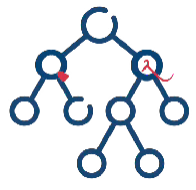
\includegraphics[height=0.9cm]{msca_logo.png}}%
  \end{center}
  \vspace{0.45cm}
  \begin{center}
    \begin{minipage}{0.1\textwidth}\centering
      \href{https://quantlet.com}{
\includegraphics[height=0.9cm]{ql_logo.png}}\end{minipage}%
    \begin{minipage}{0.78\textwidth}\centering
      {\Large\bfseries\usebeamercolor[fg]{title}\inserttitle}\par\vspace{0.25cm}
      {\large\usebeamercolor[fg]{title}\insertsubtitle}\end{minipage}%
    \begin{minipage}{0.1\textwidth}\centering
      \href{https://quantinar.com}{
\includegraphics[height=0.9cm]{qr_logo.png}}\end{minipage}
  \end{center}
  \vfill
  \hspace{0.4cm}{\bfseries\insertauthor}\par\vspace{0.12cm}
  \hspace{0.4cm}\begin{minipage}[t]{0.92\textwidth}\raggedright\footnotesize\insertinstitute\end{minipage}
  \par\vspace{0.4cm}}

% ---------------------------------------------------------------- lecture metadata
\newcommand{\nnshort}{}
\newcommand{\nnnb}{notebooks}
\newcommand{\nnrepo}{https://github.com/danpele/NEURAL_BIZ/tree/main}
% language-dependent labels (English default; \nnromanian switches to Romanian, call it before \nnlecture)
\newcommand{\txtcourse}{Neural Networks and Deep Learning}
\newcommand{\txtlecture}{Lecture}
\newcommand{\txtoutline}{Outline}
\newcommand{\txtintuition}{In one sentence:}
\newcommand{\txtjob}{In practice:}
\newcommand{\txttry}{Experiment yourself:}
\newcommand{\txtwhere}{where}
\newcommand{\txtsim}{SIMULATED DATA (teaching illustration)}
\newcommand{\txtnbsuffix}{}
\newcommand{\txtinstitute}{Bucharest University of Economic Studies (ASE), Department of Statistics and Econometrics\\
    Romanian Academy, Institute for Economic Forecasting (IPE)\\
    IDA Institute Digital Assets \textbullet\ AI4EFin \textbullet\ MSCA Digital Finance}
\newcommand{\nnromanian}{%
  \renewcommand{\txtcourse}{Rețele neuronale și deep learning}%
  \renewcommand{\txtlecture}{Cursul}%
  \renewcommand{\txtoutline}{Cuprins}%
  \renewcommand{\txtintuition}{Pe scurt:}%
  \renewcommand{\txtjob}{În practică:}%
  \renewcommand{\txttry}{Exercițiu practic:}%
  \renewcommand{\txtwhere}{unde}%
  \renewcommand{\txtsim}{DATE SIMULATE (doar pentru ilustrare)}%
  \renewcommand{\txtnbsuffix}{\string_ro}%
  \renewcommand{\txtinstitute}{Academia de Studii Economice din București (ASE), Departamentul de Statistică și Econometrie\\
    Academia Română, Institutul de Prognoză Economică (IPE)\\
    IDA Institute Digital Assets \textbullet\ AI4EFin \textbullet\ MSCA Digital Finance}}
\newcommand{\nnlecture}[2]{%
  \renewcommand{\nnshort}{\txtlecture\ #1}%
  \renewcommand{\nnnb}{notebooks/L#1\string_notebook\txtnbsuffix.ipynb}%
  \title[NN]{\txtcourse}%
  \subtitle{\txtlecture\ #1: #2}%
  \author{Prof.\ dr.\ Daniel Traian PELE}%
  \institute{\txtinstitute}%
  \date{}}

% ---------------------------------------------------------------- teaching blocks (one message per frame)
% \intuition{one plain sentence}  ->  formula with every symbol defined  ->  real-data example  ->  \manager{one line}
\newcommand{\intuition}[1]{\begin{itemize}\item {\color{MainBlue}\textbf{\txtintuition}}~#1\end{itemize}\vspace{0.6mm}}
\newcommand{\manager}[1]{\colorbox{Forest!10}{\parbox{\dimexpr\linewidth-2\fboxsep\relax}{\footnotesize
  \begin{itemize}\setlength{\itemsep}{0pt}\item \textbf{\color{Forest}\txtjob}~#1\end{itemize}}}}
% Experiment yourself: pointer to the matching notebook section
\newcommand{\tryit}[1]{{\scriptsize\href{\nnrepo/\nnnb}{%
  \raisebox{-0.15em}{
\includegraphics[height=0.85em]{ql_logo.png}}\,\textbf{\txttry}~\color{MainBlue}#1}}}
% bottom row: manager line (left) + experiment pointer (right), pinned to the bottom of the frame
\newcommand{\bottomrow}[2]{\par\vfill\noindent\begin{minipage}[b]{0.72\linewidth}#1\end{minipage}\hfill
  \begin{minipage}[b]{0.26\linewidth}\raggedleft #2\end{minipage}\par\vspace{0.5mm}}
\newcommand{\where}[1]{{\footnotesize\textbf{\txtwhere}~#1\par}}

% ---------------------------------------------------------------- helpers
% chart source line under a figure: \chartsource{Source ...; period ...}
\newcommand{\chartsource}[1]{\par\vspace{1pt}{\scriptsize\color{FooterGray}#1\par}}
% link to code: \quantlet{label}{path inside the repo}
\newcommand{\quantlet}[2]{\par\vspace{1pt}\hfill\href{\nnrepo/#2}{%
  \raisebox{-0.15em}{
\includegraphics[height=0.75em]{ql_logo.png}}\textcolor{MainBlue}{\scriptsize\ #1}}}
% inline Quantlet link for the bottom-right corner of a frame: \qlink{label}{path inside the repo}
\newcommand{\qlink}[2]{{\scriptsize\href{\nnrepo/#2}{\raisebox{-0.15em}{
\includegraphics[height=0.85em]{ql_logo.png}}\,\textcolor{MainBlue}{#1}}}}
\newcommand{\simlabel}{\colorbox{Crimson!12}{\scriptsize\bfseries\color{Crimson}\txtsim}}
\newcommand{\E}{\mathbb{E}}
\newcommand{\Var}{\operatorname{Var}}
\newcommand{\Cov}{\operatorname{Cov}}
\newcommand{\Corr}{\operatorname{Corr}}
\newcommand{\asinh}{\operatorname{asinh}}
\newcommand{\iid}{\overset{\text{i.i.d.}}{\sim}}
\newcommand{\EUR}{EUR}
% deep-learning notation (Bishop & Bishop, 2024): vectors bold lower case, matrices bold upper case
\newcommand{\R}{\mathbb{R}}
\newcommand{\vx}{\mathbf{x}}
\newcommand{\vy}{\mathbf{y}}
\newcommand{\vz}{\mathbf{z}}
\newcommand{\vh}{\mathbf{h}}
\newcommand{\vw}{\mathbf{w}}
\newcommand{\vb}{\mathbf{b}}
\newcommand{\mW}{\mathbf{W}}
\newcommand{\mX}{\mathbf{X}}
\newcommand{\btheta}{\boldsymbol{\theta}}
\newcommand{\loss}{\mathcal{L}}
\newcommand{\dataset}{\mathcal{D}}
\DeclareMathOperator*{\argmin}{arg\,min}
\DeclareMathOperator*{\argmax}{arg\,max}
\DeclareMathOperator{\softmax}{softmax}
\DeclareMathOperator{\ReLU}{ReLU}
\DeclareMathOperator{\sigm}{\sigma}

\nnlecture{2}{Training: backpropagation and optimisation}
\begin{document}
{\setbeamertemplate{headline}{}\setbeamertemplate{footline}{}
\begin{frame}\titlepage\end{frame}}
% END-FRONT-MATTER

\begin{frame}{Learning objectives}
\small
\begin{itemize}\setlength{\itemsep}{4pt}
  \item Write gradient descent (GD) as the solution method of empirical risk minimisation and explain why conditioning sets its speed.
  \item Derive backpropagation for a multilayer perceptron (MLP), compute it by hand on real data, and check it against automatic differentiation.
  \item Explain vanishing and exploding gradients and choose an initialisation that keeps the signal alive.
  \item Compare stochastic gradient descent (SGD), momentum, root mean square propagation (RMSProp), Adam and learning-rate schedules on real data, with several seeds.
  \item Train a quantile network for the 1-day value at risk (VaR) of the S\&P 500 and backtest it.
\end{itemize}
\end{frame}

% BEGIN-ABBR

\begin{frame}{Abbreviations}
\small
\vspace{-1mm}\begin{columns}[T,onlytextwidth]
\begin{column}{0.49\textwidth}{\scriptsize\renewcommand{\arraystretch}{0.96}\begin{tabular}{@{}>{\bfseries}l@{\ \ }p{0.74\linewidth}@{}}AdamW & Adam with decoupled weight decay\\
CPU & central processing unit\\
ES & expected shortfall\\
EWMA & exponentially weighted moving average\\
GD & gradient descent\\
GPU & graphics processing unit\\
LLM & large language model\\
MLP & multilayer perceptron\\
MPS & Metal Performance Shaders (Apple GPU back-end of PyTorch)\\\end{tabular}}\end{column}
\begin{column}{0.49\textwidth}{\scriptsize\renewcommand{\arraystretch}{0.96}\begin{tabular}{@{}>{\bfseries}l@{\ \ }p{0.74\linewidth}@{}}MSE & mean squared error\\
OpenML & Open Machine Learning platform\\
PCA & principal component analysis\\
PR-AUC & area under the precision-recall curve\\
ReLU & rectified linear unit\\
RMSProp & root mean square propagation\\
SGD & stochastic gradient descent\\
ULB & Université libre de Bruxelles\\
VaR & value at risk\\\end{tabular}}\end{column}
\end{columns}
\end{frame}

% END-ABBR


\section{From the loss to the gradient}

\begin{frame}{Training a network is a high-dimensional, non-convex minimisation}
\small
\intuition{we cannot solve for the weights as in least squares; we walk downhill on the loss, one step at a time.}
\[ \hat\btheta=\argmin_{\btheta\in\R^{P}}\ \loss(\btheta),\qquad \loss(\btheta)=\frac1n\sum_{i=1}^n\ell\big(y_i,f(\vx_i;\btheta)\big),\qquad \btheta_{t+1}=\btheta_t-\eta\,\nabla\loss(\btheta_t) \]
{\footnotesize\begin{itemize}\setlength{\itemsep}{0pt}
  \item \textbf{\txtwhere}
    \begin{itemize}\setlength{\itemsep}{0pt}
      \item $P$ the number of parameters, $\eta>0$ the learning rate, $\nabla\loss$ the gradient, computed by backpropagation (Section 2)
    \end{itemize}
\end{itemize}\par}
\begin{itemize}\setlength{\itemsep}{2pt}
  \item Why it works: $\loss(\btheta-\eta\mathbf g)=\loss(\btheta)-\eta\|\mathbf g\|^2+O(\eta^2)$, so a small step against the gradient lowers the loss.
  \item The MLP 64-64 of this lecture has 4\,801 parameters on 12\,384 training block groups
    \begin{itemize}\setlength{\itemsep}{0pt}
      \item Models in production have millions.
    \end{itemize}
  \item Two questions: how to get $\nabla\loss$ cheaply and how to step well.
\end{itemize}
\par\vfill\manager{every model of this course is trained by some variant of this one-line update.}\par\vspace{0.5mm}
\par\vfill\noindent{\scriptsize\color{FooterGray}(Bishop \& Bishop, 2024, ch.~7)}\par\vspace{0.5mm}
\end{frame}

\begin{frame}{The data of this lecture: houses, card payments and the S\&P 500}
\small
{\scriptsize\renewcommand{\arraystretch}{1.05}\setlength{\tabcolsep}{4pt}
\begin{tabular}{@{}p{0.25\textwidth}rp{0.27\textwidth}p{0.34\textwidth}@{}}\toprule
Dataset & Rows & Task & Split \\ \midrule
California housing & 20\,640 & regression: house value & random 60/20/20: 12\,384 / 4\,128 / 4\,128 \\
Card fraud (sample) & 28\,924 & classification: fraud & by time: first 60\,\% train, next 20\,\% validation, last 20\,\% test \\
S\&P 500 & 1\,716 & 1\,\% quantile of the next-day return & by time: train to 2016, validation 2017--2019, test from 2020 \\
\bottomrule\end{tabular}}
\par\vspace{0.5mm}{\scriptsize \begin{itemize}\setlength{\itemsep}{0pt}
  \item Fraud: Université libre de Bruxelles (ULB) and Worldline data, on the Open Machine Learning platform (OpenML); all 492 frauds and a 10\,\% sample of legitimate payments; inputs V1--V28 are principal component analysis (PCA) scores released by the bank.
  \item Weights restore the full-data fraud rate of 0.173\,\% in every precision-type metric; S\&P 500: daily log returns in \%, test rows = forecast days.
\end{itemize}}
\par\vfill\manager{time series and fraud are split in time order: the model never sees the future.}\par\vspace{0.5mm}
\par\vfill\noindent{\scriptsize\color{FooterGray}(Pace \& Barry, 1997; Dal Pozzolo et al., 2015)}\hfill\tryit{notebook \S1}\par\vspace{0.5mm}
\end{frame}

\begin{frame}{Badly scaled inputs turn the loss into a narrow valley}
\small
\intuition{the real loss of $\hat y=a+b\cdot\text{income}$ on California: gradient descent zig-zags on raw income and goes straight on standardised income.}
\begin{center}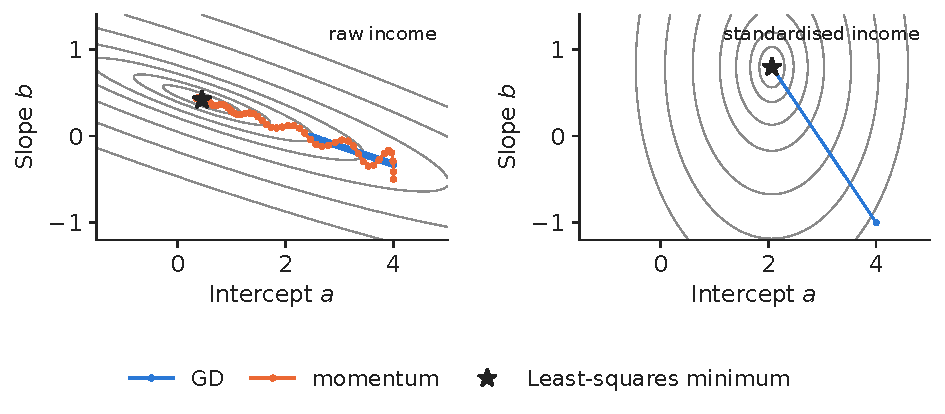
\includegraphics[width=\textwidth,height=0.354\textheight,keepaspectratio]{charts/en/gd_paths.pdf}\end{center}\vspace{-3mm}
\chartsource{Source: StatLib, California housing, 1990 census (Pace and Barry, 1997). Data: 20,640 block groups, 1990 census.}
\vspace{0.5mm}
\begin{itemize}\setlength{\itemsep}{0pt}
  \item Condition number $\kappa=\lambda_{\max}/\lambda_{\min}$ of the Hessian: 104.3 raw, 1 standardised
    \begin{itemize}\setlength{\itemsep}{0pt}
      \item After 60 steps: mean squared error (MSE) 1.486 (GD, raw), 0.704 (momentum, raw), 0.701 (GD, standardised)
      \item Minimum 0.701.
    \end{itemize}
\end{itemize}
\par\vfill\manager{standardise every input on the training set before training any network.}\par\vspace{0.5mm}
\par\vfill\noindent{\scriptsize\color{FooterGray}(own computation)}\hfill\qlink{NN\_L2\_gd\_paths}{Quantlets/L2/NN_L2_gd_paths}\par\vspace{0.5mm}
\end{frame}

\begin{frame}{On a quadratic, the step size must stay below $2/\lambda_{\max}$}
\small
\intuition{along each eigen-direction of the Hessian, gradient descent multiplies the error by $(1-\eta\lambda_k)$.}
\[ \loss(\btheta)=\loss^*+\tfrac12(\btheta-\btheta^*)^\top\mathbf H(\btheta-\btheta^*)\ \Rightarrow\ \btheta_{t}-\btheta^*=(\mathbf I-\eta\mathbf H)^t(\btheta_0-\btheta^*),\qquad |1-\eta\lambda_k|<1\iff 0<\eta<\frac{2}{\lambda_{\max}} \]
{\footnotesize\begin{itemize}\setlength{\itemsep}{0pt}
  \item \textbf{\txtwhere}
    \begin{itemize}\setlength{\itemsep}{0pt}
      \item $\mathbf H$ the Hessian with eigenvalues $\lambda_{\min}\le\dots\le\lambda_{\max}$, $\btheta^*$ the minimum
    \end{itemize}
\end{itemize}\par}
\begin{itemize}\setlength{\itemsep}{2pt}
  \item With the best fixed step the error shrinks by $(\kappa-1)/(\kappa+1)$ per step: slow when $\kappa$ is large.
  \item Raw income: $\kappa=$ 104.3, so the step $1/\lambda_{\max}=$ 0.0258 barely moves the flat direction.
  \item Networks are not quadratic, but near a minimum they behave like one: the same limit explains divergence at large $\eta$.
\end{itemize}
\par\vfill\manager{if the loss explodes in the first epochs, divide the learning rate by 3 before changing anything else.}\par\vspace{0.5mm}
\par\vfill\noindent{\scriptsize\color{FooterGray}(Bishop \& Bishop, 2024, ch.~7)}\par\vspace{0.5mm}
\end{frame}


\section{Backpropagation}

\begin{frame}{Backpropagation is the chain rule, applied from the loss backwards}
\small
\intuition{each node of the computational graph multiplies the incoming gradient by its own local derivative and passes it on.}
\[ \vz^{(l)}=\mW^{(l)}\vh^{(l-1)}+\vb^{(l)},\quad \vh^{(l)}=a(\vz^{(l)});\qquad \boldsymbol\delta^{(L)}=\frac{\partial\ell}{\partial\vz^{(L)}},\quad \boldsymbol\delta^{(l)}=\big(\mW^{(l+1)\top}\boldsymbol\delta^{(l+1)}\big)\odot a'(\vz^{(l)}) \]
\[ \frac{\partial\ell}{\partial\mW^{(l)}}=\boldsymbol\delta^{(l)}\,\vh^{(l-1)\top},\qquad \frac{\partial\ell}{\partial\vb^{(l)}}=\boldsymbol\delta^{(l)} \]
{\footnotesize\begin{itemize}\setlength{\itemsep}{0pt}
  \item \textbf{\txtwhere}
    \begin{itemize}\setlength{\itemsep}{0pt}
      \item $\boldsymbol\delta^{(l)}$ the error signal of layer $l$, $\odot$ the element-wise product, $a'$ the derivative of the activation
    \end{itemize}
\end{itemize}\par}
\begin{itemize}\setlength{\itemsep}{2pt}
  \item Output error: $\hat y-y$ (squared loss), $p-y$ (sigmoid with cross-entropy, Lecture 1).
  \item Weight gradient = error of the layer times its input, as in the logistic gradient.
\end{itemize}
\par\vfill\manager{the forward pass must store $\vz^{(l)}$ and $\vh^{(l)}$: this memory, not arithmetic, limits batch size on a graphics processing unit (GPU).}\par\vspace{0.5mm}
\par\vfill\noindent{\scriptsize\color{FooterGray}(Rumelhart, Hinton \& Williams, 1986)}\par\vspace{0.5mm}
\end{frame}

\begin{frame}{Backpropagation by hand on one real block group}
\small
\intuition{two standardised inputs, two rectified linear units (ReLU), one linear output and the loss $\ell=\tfrac12(\hat y-y)^2$.}
\begin{columns}[T,onlytextwidth]
\begin{column}{0.48\textwidth}
{\scriptsize\renewcommand{\arraystretch}{1.05}\setlength{\tabcolsep}{4pt}
\begin{tabular}{@{}lrr@{}}\toprule
Forward & unit 1 & unit 2 \\ \midrule
input $x$ (income, latitude) & \ensuremath{-}0.21 & \ensuremath{-}0.67 \\
weights $\mW^{(1)}$, row 1 / row 2 & \ensuremath{-}0.28, \ensuremath{-}0.56 & 0.50, \ensuremath{-}0.02 \\
$z=\mW^{(1)}x$ & 0.433 & \ensuremath{-}0.093 \\
$h=\max(0,z)$ & 0.433 & 0.000 \\
output weights $w^{(2)}$ & \ensuremath{-}0.87 & \ensuremath{-}0.19 \\
$\hat y=w^{(2)\top}h$; $y$ & \ensuremath{-}0.377 & 2.067 \\
\bottomrule\end{tabular}}
\end{column}
\begin{column}{0.49\textwidth}
{\scriptsize\renewcommand{\arraystretch}{1.05}\setlength{\tabcolsep}{4pt}
\begin{tabular}{@{}lrr@{}}\toprule
Backward & unit 1 & unit 2 \\ \midrule
$\delta^{(2)}=\hat y-y$ & \ensuremath{-}2.444 &  \\
$\partial\ell/\partial w^{(2)}=\delta^{(2)}h$ & \ensuremath{-}1.059 & \ensuremath{-}0.000 \\
$\delta^{(1)}=\delta^{(2)}w^{(2)}\odot\mathbb 1\{z>0\}$ & 2.126 & 0.000 \\
$\partial\ell/\partial W^{(1)}_{k1}=\delta^{(1)}_kx_1$ & \ensuremath{-}0.453 & \ensuremath{-}0.000 \\
$\partial\ell/\partial W^{(1)}_{k2}=\delta^{(1)}_kx_2$ & \ensuremath{-}1.419 & \ensuremath{-}0.000 \\
\bottomrule\end{tabular}}
\end{column}
\end{columns}\begin{itemize}\setlength{\itemsep}{2pt}
  \item Unit 2 is switched off ($z_2<0$): it passes no gradient, so its weights do not move on this example.
  \item PyTorch autograd gives the same gradients (largest difference 0.0).
\end{itemize}
\par\vfill\manager{a ReLU unit that is off for every customer never learns again: watch the share of dead units.}\par\vspace{0.5mm}
\par\vfill\noindent{\scriptsize\color{FooterGray}(own computation)}\hfill\tryit{notebook \S2}\par\vspace{0.5mm}
\end{frame}

\begin{frame}{Reverse mode costs about one extra forward pass, whatever the number of weights}
\small
\intuition{one backward sweep gives all $P$ partial derivatives of a scalar loss; finite differences would need $P$ extra passes.}
\[ \text{cost}\big(\nabla_{\btheta}\loss\big)\ \le\ c\cdot\text{cost}\big(\loss\big),\ \ c\approx 2\text{--}3;\qquad \frac{\partial\loss}{\partial\theta_j}\approx\frac{\loss(\btheta+\epsilon\mathbf e_j)-\loss(\btheta-\epsilon\mathbf e_j)}{2\epsilon} \]
\begin{itemize}\setlength{\itemsep}{2pt}
  \item Forward mode (dual numbers) is cheap for few inputs and many outputs
    \begin{itemize}\setlength{\itemsep}{0pt}
      \item Reverse mode for many inputs (weights) and one output (loss).
    \end{itemize}
  \item Gradient check on our MLP 64-64: 30 random weights, central differences with $\epsilon=10^{-6}$ in double precision, largest relative error $7.0\times10^{-7}$.
  \item PyTorch records the graph during the forward pass
    \begin{itemize}\setlength{\itemsep}{0pt}
      \item \texttt{loss.backward()} walks it in reverse.
    \end{itemize}
\end{itemize}
\par\vfill\manager{when you write a custom layer or loss, run a gradient check once before trusting it.}\par\vspace{0.5mm}
\par\vfill\noindent{\scriptsize\color{FooterGray}(Baydin et al., 2018; Paszke et al., 2019)}\hfill\tryit{notebook \S2}\par\vspace{0.5mm}
\end{frame}

\begin{frame}{Vanishing gradients in deep sigmoid networks}
\small
\intuition{the backward signal is a product of Jacobians; with $\sigma'\le1/4$ it shrinks at every layer.}
\vspace{-1mm}\[ \frac{\partial\ell}{\partial\vh^{(l)}}=\Big(\prod_{k=l+1}^{L}\mW^{(k)\top}\operatorname{diag}\big(a'(\vz^{(k)})\big)\Big)\frac{\partial\ell}{\partial\vh^{(L)}} \]\vspace{-2mm}
\begin{center}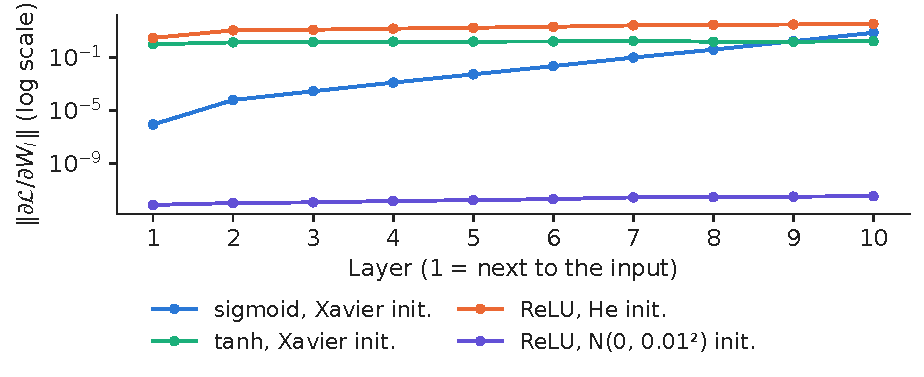
\includegraphics[width=\textwidth,height=0.320\textheight,keepaspectratio]{charts/en/vanishing.pdf}\end{center}\vspace{-3mm}
\chartsource{Source: StatLib, California housing, 1990 census (Pace and Barry, 1997). Data: 10 hidden layers of 64 units, one batch of 512 training block groups, 5 seeds.}
\vspace{0.5mm}
\begin{itemize}\setlength{\itemsep}{0pt}
  \item 10 hidden layers, one real batch: first/last layer gradient norm $8.5\times10^{-7}$ vs $7.5\times10^{0}$ with sigmoids
    \begin{itemize}\setlength{\itemsep}{0pt}
      \item $3.1\times10^{0}$ vs $3.5\times10^{1}$ with ReLU and He initialisation.
    \end{itemize}
\end{itemize}
\par\vfill\manager{deep nets need ReLU-type activations, a scaled initialisation and, later, normalisation (Lecture 3).}\par\vspace{0.5mm}
\par\vfill\noindent{\scriptsize\color{FooterGray}(own computation)}\hfill\qlink{NN\_L2\_vanishing}{Quantlets/L2/NN_L2_vanishing}\par\vspace{0.5mm}
\end{frame}

\begin{frame}{Initialisation that keeps the variance of the signal constant across layers}
\small
\intuition{too small and the signal vanishes, too large and it explodes; the right scale depends on the fan-in and on the activation.}
\[ \Var(z_j^{(l)})=n_{l-1}\Var(W)\,\E\big[(h^{(l-1)})^2\big]\ \Rightarrow\ \underbrace{\Var(W)=\frac{2}{n_{l-1}+n_l}}_{\text{Xavier (tanh, sigmoid)}},\qquad \underbrace{\Var(W)=\frac{2}{n_{l-1}}}_{\text{He (ReLU)}} \]
{\footnotesize\begin{itemize}\setlength{\itemsep}{0pt}
  \item \textbf{\txtwhere}
    \begin{itemize}\setlength{\itemsep}{0pt}
      \item $n_{l-1}$ the fan-in, $n_l$ the fan-out of layer $l$, for ReLU, $\E[h^2]=\tfrac12\Var(z)$, hence the factor 2
    \end{itemize}
\end{itemize}\par}
\begin{itemize}\setlength{\itemsep}{2pt}
  \item Weights $\mathcal N(0,0.01^2)$ in our 10-layer ReLU net: first-layer gradient norm $6.9\times10^{-13}$, i.e.\ no learning at all.
  \item Never initialise all weights equal: every unit would learn the same thing.
\end{itemize}
\par\vfill\manager{PyTorch's defaults are close to these rules
    \begin{itemize}\setlength{\itemsep}{0pt}
      \item Set He initialisation explicitly for deep ReLU nets.
    \end{itemize}}\par\vspace{0.5mm}
\par\vfill\noindent{\scriptsize\color{FooterGray}(Glorot \& Bengio, 2010; He et al., 2015)}\hfill\tryit{notebook \S3}\par\vspace{0.5mm}
\end{frame}


\section{Stochastic optimisation}

\begin{frame}{A mini-batch gives an unbiased, noisy gradient at a fraction of the cost}
\small
\intuition{averaging the gradient over $B$ random examples is enough to know roughly which way is down.}
\[ \mathbf g_t=\frac1B\sum_{i\in\mathcal B_t}\nabla\ell_i(\btheta_t),\qquad \E[\mathbf g_t]=\nabla\loss(\btheta_t),\qquad \Var(\mathbf g_t)\approx\frac{1}{B}\Big(1-\frac{B}{n}\Big)\Sigma(\btheta_t) \]
{\footnotesize\begin{itemize}\setlength{\itemsep}{0pt}
  \item \textbf{\txtwhere}
    \begin{itemize}\setlength{\itemsep}{0pt}
      \item $\mathcal B_t$ a random batch of size $B$, $\Sigma$ the covariance of the per-example gradients, one epoch $=\lceil n/B\rceil$ steps
    \end{itemize}
\end{itemize}\par}
\begin{itemize}\setlength{\itemsep}{2pt}
  \item Robbins--Monro: with $\sum_t\eta_t=\infty$ and $\sum_t\eta_t^2<\infty$, SGD converges to a stationary point.
  \item The noise is not only a cost: it helps to leave sharp minima, which tend to generalise worse (Keskar et al., 2017).
\end{itemize}
\par\vfill\manager{batches of 32--256 are the usual compromise between noise, speed and memory.}\par\vspace{0.5mm}
\par\vfill\noindent{\scriptsize\color{FooterGray}(Robbins \& Monro, 1951)}\hfill\tryit{notebook \S4}\par\vspace{0.5mm}
\end{frame}

\begin{frame}{Effect of the learning rate on training}
\small
\intuition{plain SGD on an MLP 64-64, 30 epochs, batches of 128, for nine learning rates and three seeds.}
\begin{center}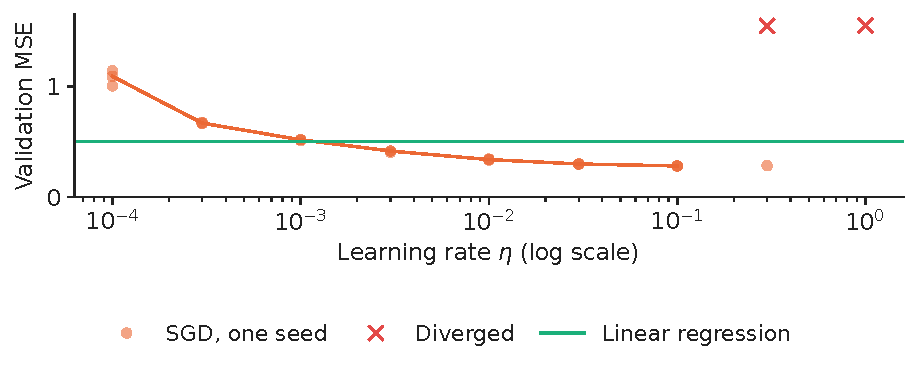
\includegraphics[width=\textwidth,height=0.405\textheight,keepaspectratio]{charts/en/lr_sweep.pdf}\end{center}\vspace{-3mm}
\chartsource{Source: StatLib, California housing, 1990 census (Pace and Barry, 1997). Data: 12,384 training and 4,128 validation block groups; 30 epochs.}
\vspace{0.5mm}
\begin{itemize}\setlength{\itemsep}{0pt}
  \item Validation MSE 1.093 at $\eta=10^{-4}$ (worse than linear regression, 0.500), 0.281 at $\eta=$ 0.1
    \begin{itemize}\setlength{\itemsep}{0pt}
      \item From $\eta=$ 0.3 at least one seed diverges.
    \end{itemize}
\end{itemize}
\par\vfill\manager{tune the learning rate first, on a log grid, before any other hyperparameter.}\par\vspace{0.5mm}
\par\vfill\noindent{\scriptsize\color{FooterGray}(own computation)}\hfill\qlink{NN\_L2\_lr\_sweep}{Quantlets/L2/NN_L2_lr_sweep}\par\vspace{0.5mm}
\end{frame}

\begin{frame}{Effect of batch size: progress per epoch and per second}
\small
\intuition{Adam with learning rate 0.001, 40 epochs, batch sizes 16, 128 and 1,024.}
\begin{center}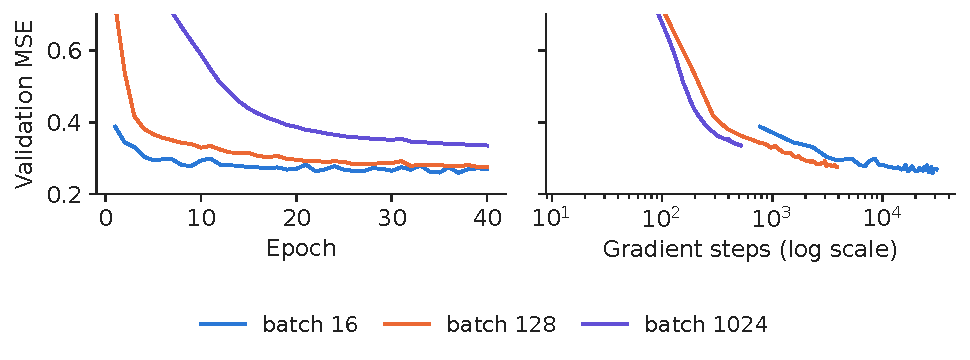
\includegraphics[width=\textwidth,height=0.480\textheight,keepaspectratio]{charts/en/batch_size.pdf}\end{center}\vspace{-3mm}
\chartsource{Source: StatLib, California housing, 1990 census (Pace and Barry, 1997). Data: Adam, learning rate 0.001, 40 epochs.}
\vspace{0.5mm}
\begin{itemize}\setlength{\itemsep}{0pt}
  \item After 5 epochs: validation MSE 0.294 (batch 16), 0.367 (128), 0.870 (1,024)
    \begin{itemize}\setlength{\itemsep}{0pt}
      \item Wall time for 40 epochs on one processor thread: 25.8, 3.7 and 1.0 seconds.
    \end{itemize}
\end{itemize}
\par\vfill\manager{compare training budgets in gradient steps or seconds, not in epochs.}\par\vspace{0.5mm}
\par\vfill\noindent{\scriptsize\color{FooterGray}(own computation)}\hfill\qlink{NN\_L2\_batch\_size}{Quantlets/L2/NN_L2_batch_size}\par\vspace{0.5mm}
\end{frame}

\begin{frame}{Momentum: a running average of past gradients}
\small
\intuition{zig-zag components cancel in the average, the consistent downhill component accumulates.}
\[ \mathbf v_{t+1}=\beta\,\mathbf v_t+\mathbf g_t,\qquad \btheta_{t+1}=\btheta_t-\eta\,\mathbf v_{t+1};\qquad \text{Nesterov:}\ \mathbf g_t=\nabla\loss(\btheta_t-\eta\beta\mathbf v_t) \]
{\footnotesize\begin{itemize}\setlength{\itemsep}{0pt}
  \item \textbf{\txtwhere}
    \begin{itemize}\setlength{\itemsep}{0pt}
      \item $\mathbf v$ the velocity, $\beta\in[0,1)$ the momentum, usually 0.9, the effective step on a constant slope is $\eta/(1-\beta)$, ten times $\eta$
    \end{itemize}
\end{itemize}\par}
\begin{itemize}\setlength{\itemsep}{2pt}
  \item On a quadratic, the best momentum improves the contraction from $\frac{\kappa-1}{\kappa+1}$ to $\frac{\sqrt\kappa-1}{\sqrt\kappa+1}$ (Polyak, 1964).
  \item Raw-income regression after 60 steps: MSE 0.704 with momentum against 1.486 for plain GD.
\end{itemize}
\par\vfill\manager{SGD with momentum 0.9 is still the default for very large vision models.}\par\vspace{0.5mm}
\par\vfill\noindent{\scriptsize\color{FooterGray}(Polyak, 1964)}\hfill\tryit{notebook \S5}\par\vspace{0.5mm}
\end{frame}

\begin{frame}{Adaptive methods give each weight its own step size}
\small
\intuition{divide the step by a running measure of how large that weight's gradients have been.}
\[ \text{AdaGrad: } s_t=s_{t-1}+g_t^2;\qquad \text{RMSProp: } s_t=\rho\,s_{t-1}+(1-\rho)\,g_t^2;\qquad \theta_{t+1}=\theta_t-\frac{\eta}{\sqrt{s_t}+\epsilon}\,g_t \]
{\footnotesize\begin{itemize}\setlength{\itemsep}{0pt}
  \item \textbf{\txtwhere}
    \begin{itemize}\setlength{\itemsep}{0pt}
      \item All operations element by element, $\rho\approx0.99$, $\epsilon\approx10^{-8}$ avoids division by zero
    \end{itemize}
\end{itemize}\par}
\begin{itemize}\setlength{\itemsep}{2pt}
  \item AdaGrad's sum only grows, so its steps shrink to zero: good for sparse features, too slow for deep nets (Duchi, Hazan \& Singer, 2011).
  \item Root mean square propagation (RMSProp) forgets old gradients exponentially, so the step adapts to the current region (Tieleman \& Hinton, 2012).
  \item Rescaling per weight partly undoes bad conditioning: rarely updated or flat directions get larger steps.
\end{itemize}
\par\vfill\manager{adaptive methods are less sensitive to the learning rate, which makes them a safe first choice.}\par\vspace{0.5mm}
\par\vfill\noindent{\scriptsize\color{FooterGray}}\hfill\tryit{notebook \S5}\par\vspace{0.5mm}
\end{frame}

\begin{frame}{Adam: momentum, RMSProp and a bias correction}
\small
\intuition{keep moving averages of the gradient and of its square, correct them for starting at zero, and step by their ratio.}
\[ m_t=\beta_1m_{t-1}+(1-\beta_1)g_t,\quad v_t=\beta_2v_{t-1}+(1-\beta_2)g_t^2,\quad \hat m_t=\frac{m_t}{1-\beta_1^t},\ \hat v_t=\frac{v_t}{1-\beta_2^t},\quad \theta_{t+1}=\theta_t-\eta\,\frac{\hat m_t}{\sqrt{\hat v_t}+\epsilon} \]
{\footnotesize\begin{itemize}\setlength{\itemsep}{0pt}
  \item \textbf{\txtwhere}
    \begin{itemize}\setlength{\itemsep}{0pt}
      \item Defaults $\beta_1=0.9$, $\beta_2=0.999$, $\epsilon=10^{-8}$, $\eta=10^{-3}$, $m_0=v_0=0$, hence the correction (appendix)
    \end{itemize}
\end{itemize}\par}
\begin{itemize}\setlength{\itemsep}{2pt}
  \item The step is roughly bounded by $\eta$ per weight, whatever the scale of the loss: easy to tune.
  \item Adam with decoupled weight decay (AdamW) shrinks weights directly, $\theta\leftarrow\theta-\eta\lambda\theta$, instead of adding $\lambda\theta$ to $g_t$ (Loshchilov \& Hutter, 2019; Lecture 3).
\end{itemize}
\par\vfill\manager{start with AdamW and $\eta=10^{-3}$
    \begin{itemize}\setlength{\itemsep}{0pt}
      \item Move to tuned SGD with momentum only if it pays out of sample.
    \end{itemize}}\par\vspace{0.5mm}
\par\vfill\noindent{\scriptsize\color{FooterGray}(Kingma \& Ba, 2015)}\hfill\tryit{notebook \S5}\par\vspace{0.5mm}
\end{frame}

\begin{frame}{On California housing, tuned optimisers reach similar errors and adaptive methods converge more reliably}
\small
\intuition{best of three learning rates per optimiser (on validation), mean of 5 new seeds.}
\begin{center}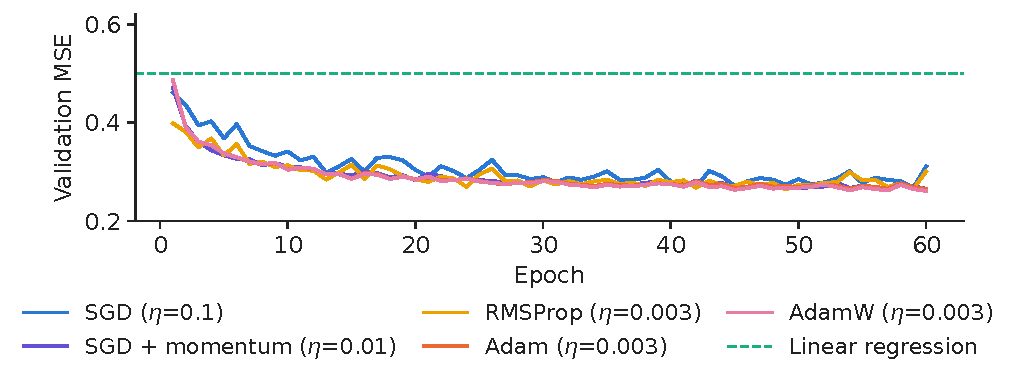
\includegraphics[width=\textwidth,height=0.376\textheight,keepaspectratio]{charts/en/optimizers.pdf}\end{center}\vspace{-3mm}
\chartsource{Source: StatLib, California housing, 1990 census (Pace and Barry, 1997). Data: 12,384 training and 4,128 validation block groups.}
\vspace{0.5mm}
\begin{itemize}\setlength{\itemsep}{0pt}
  \item Validation MSE after 10 epochs: SGD 0.342, momentum 0.310, RMSProp 0.313, Adam 0.305, AdamW 0.304
    \begin{itemize}\setlength{\itemsep}{0pt}
      \item Linear regression 0.500.
    \end{itemize}
\end{itemize}
\par\vfill\manager{the network halves the error of the linear benchmark whatever the optimiser.}\par\vspace{0.5mm}
\par\vfill\noindent{\scriptsize\color{FooterGray}(own computation)}\hfill\qlink{NN\_L2\_optimizers}{Quantlets/L2/NN_L2_optimizers}\par\vspace{0.5mm}
\end{frame}

\begin{frame}{Across seeds, Adam and AdamW are far more stable than plain SGD}
\small
\intuition{test MSE of 5 seeds per optimiser; a single run would have ranked them by luck.}
\begin{center}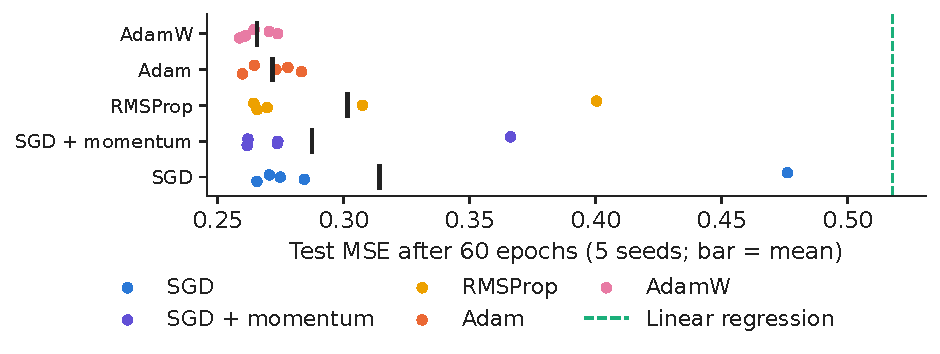
\includegraphics[width=\textwidth,height=0.478\textheight,keepaspectratio]{charts/en/optimizer_seeds.pdf}\end{center}\vspace{-3mm}
\chartsource{Source: StatLib, California housing, 1990 census (Pace and Barry, 1997). Data: 4,128 test block groups.}
\vspace{0.5mm}
\begin{itemize}\setlength{\itemsep}{0pt}
  \item Test MSE mean (standard deviation): SGD 0.314 (0.091), Adam 0.272 (0.010), AdamW 0.266 (0.006)
    \begin{itemize}\setlength{\itemsep}{0pt}
      \item Paired $t$-test SGD vs Adam: $t=$ 1.01, $p=$ 0.371.
    \end{itemize}
\end{itemize}
\par\vfill\manager{the mean gain is not significant with 5 seeds, but the risk of a bad run is much lower with Adam.}\par\vspace{0.5mm}
\par\vfill\noindent{\scriptsize\color{FooterGray}(own computation)}\hfill\qlink{NN\_L2\_optimizer\_seeds}{Quantlets/L2/NN_L2_optimizer_seeds}\par\vspace{0.5mm}
\end{frame}

\begin{frame}{Learning-rate schedules: step, cosine and one-cycle}
\small
\intuition{explore with a large step, then reduce it so that the noise of SGD settles into a minimum.}
\[ \text{step: }\eta_t=\eta_0\gamma^{\lfloor t/s\rfloor};\qquad \text{cosine: }\eta_t=\tfrac{\eta_0}{2}\Big(1+\cos\frac{\pi t}{T}\Big) \]
\[ \text{one-cycle: linear warm-up to }\eta_0,\text{ then cosine to }\approx0 \]
{\footnotesize\begin{itemize}\setlength{\itemsep}{0pt}
  \item \textbf{\txtwhere}
    \begin{itemize}\setlength{\itemsep}{0pt}
      \item $\eta_0$ the peak rate, $\gamma$ the decay factor every $s$ steps, $T$ the total number of steps
    \end{itemize}
\end{itemize}\par}
\begin{itemize}\setlength{\itemsep}{2pt}
  \item Cosine annealing (Loshchilov \& Hutter, 2017) and one-cycle (Smith \& Topin, 2019) need only the peak rate and the budget.
  \item Warm-up protects the first steps, when Adam's second-moment estimates and batch statistics are still unreliable.
\end{itemize}
\par\vfill\manager{a cosine schedule over the planned number of epochs is a safe default.}\par\vspace{0.5mm}
\par\vfill\noindent{\scriptsize\color{FooterGray}(Bishop \& Bishop, 2024, ch.~7)}\hfill\tryit{notebook \S6}\par\vspace{0.5mm}
\end{frame}

\begin{frame}{Decaying the learning rate lowers the final error}
\small
\intuition{SGD with momentum 0.9 and peak rate 0.01; left the schedules, right the validation MSE (mean of 3 seeds).}
\begin{center}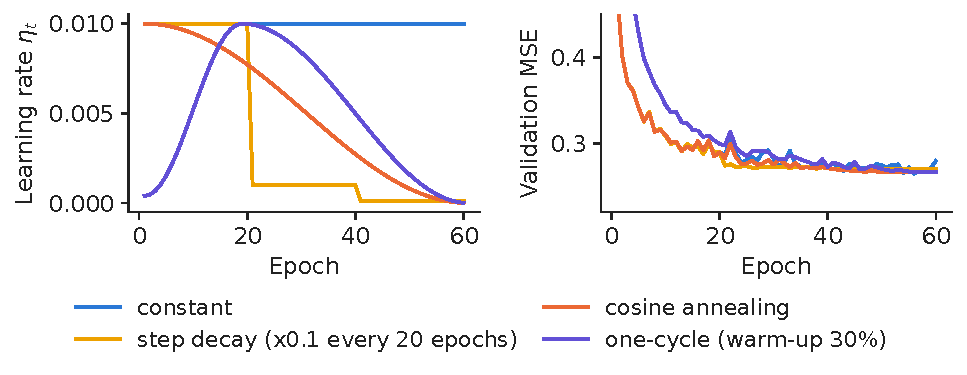
\includegraphics[width=\textwidth,height=0.426\textheight,keepaspectratio]{charts/en/schedules.pdf}\end{center}\vspace{-3mm}
\chartsource{Source: StatLib, California housing, 1990 census (Pace and Barry, 1997). Data: SGD with momentum 0.9, peak rate 0.01, 3 seeds.}
\vspace{0.5mm}
\begin{itemize}\setlength{\itemsep}{0pt}
  \item Final validation MSE: constant 0.279, step 0.270, cosine 0.266, one-cycle 0.266
    \begin{itemize}\setlength{\itemsep}{0pt}
      \item Test 0.286 vs 0.265 (constant vs cosine).
    \end{itemize}
\end{itemize}
\par\vfill\manager{the schedule is a cheap gain: same model, same budget, lower error.}\par\vspace{0.5mm}
\par\vfill\noindent{\scriptsize\color{FooterGray}(own computation)}\hfill\qlink{NN\_L2\_schedules}{Quantlets/L2/NN_L2_schedules}\par\vspace{0.5mm}
\end{frame}

\begin{frame}{On card fraud, the optimiser determines the speed of learning}
\small
\intuition{MLP 64-64 trained on the first 60\,\% of the two days, scored on the next 20\,\%.}
\begin{center}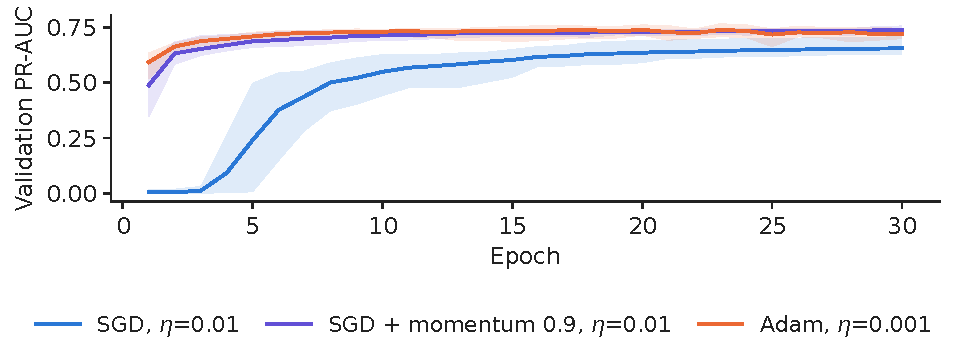
\includegraphics[width=\textwidth,height=0.420\textheight,keepaspectratio]{charts/en/fraud_optimizers.pdf}\end{center}\vspace{-3mm}
\chartsource{Source: ULB Machine Learning Group and Worldline, credit-card transactions (OpenML 1597). Data: September 2013, 2 days; train = first 33.4 hours, validation to hour 40.3; 5 seeds.}
\vspace{0.5mm}
\begin{itemize}\setlength{\itemsep}{0pt}
  \item Area under the precision-recall curve (PR-AUC) after 1 epoch: SGD 0.004, momentum 0.488, Adam 0.592 (test hours: 0.786, 0.823, 0.803).
\end{itemize}
\par\vfill\manager{with a rare class, plain SGD needs many epochs, momentum or Adam only one.}\par\vspace{0.5mm}
\par\vfill\noindent{\scriptsize\color{FooterGray}(own computation)}\hfill\qlink{NN\_L2\_fraud\_optimizers}{Quantlets/L2/NN_L2_fraud_optimizers}\par\vspace{0.5mm}
\end{frame}

\begin{frame}{Comparison of optimisers}
\small
{\scriptsize\renewcommand{\arraystretch}{1.05}\setlength{\tabcolsep}{4pt}
\begin{tabular}{@{}p{0.15\textwidth}p{0.37\textwidth}p{0.17\textwidth}p{0.24\textwidth}@{}}\toprule
Method & Update & Extra memory & Use when \\ \midrule
SGD & $\theta-\eta g$ & none & large vision models, tuned schedule \\
Momentum & $v\leftarrow\beta v+g$, $\theta-\eta v$ & 1 vector & ill-conditioned losses \\
RMSProp & $\theta-\eta g/\sqrt{s}$, $s$ = avg$(g^2)$ & 1 vector & recurrent nets, non-stationary losses \\
Adam & $\theta-\eta\hat m/(\sqrt{\hat v}+\epsilon)$ & 2 vectors & default first choice \\
AdamW & Adam $+$ decay $(1-\eta\lambda)\theta$ & 2 vectors & whenever weight decay is used \\
\bottomrule\end{tabular}}
\par\vspace{0.5mm}{\scriptsize \begin{itemize}\setlength{\itemsep}{0pt}
  \item Memory is per weight: Adam stores two extra numbers for every parameter, which matters for very large models.
\end{itemize}}
\par\vfill\manager{choose by budget and stability
    \begin{itemize}\setlength{\itemsep}{0pt}
      \item On our data the tuned optimisers end close, Adam and AdamW are the most stable.
    \end{itemize}}\par\vspace{0.5mm}
\par\vfill\noindent{\scriptsize\color{FooterGray}(Bishop \& Bishop, 2024, ch.~7)}\par\vspace{0.5mm}
\end{frame}


\section{Case study: value at risk with a quantile network}

\begin{frame}{The pinball loss turns any network into a quantile forecaster}
\small
\intuition{penalise returns below the forecast $1-\tau$ times more than returns above it, and the minimiser is the $\tau$-quantile.}
\[ \mathrm{VaR}^{\tau}_{t+1}=-q_{\tau}(r_{t+1}\mid\mathcal F_t),\qquad \rho_\tau(u)=u\big(\tau-\mathbb 1\{u<0\}\big),\qquad \hat q=\argmin_{q}\ \E\,\rho_\tau(r-q) \]
{\footnotesize\begin{itemize}\setlength{\itemsep}{0pt}
  \item \textbf{\txtwhere}
    \begin{itemize}\setlength{\itemsep}{0pt}
      \item $r_{t+1}$ the next-day log return in \%, $\mathcal F_t$ the information up to day $t$, $\tau=1\,\%$ for a 99\,\% VaR
    \end{itemize}
\end{itemize}\par}
\begin{itemize}\setlength{\itemsep}{2pt}
  \item Network: inputs $r_t$, $|r_t|$, 5-day mean, 5-, 22- and 66-day volatility
    \begin{itemize}\setlength{\itemsep}{0pt}
      \item MLP 32-32 trained with Adam on $\frac1n\sum\rho_\tau(r_{t+1}-\hat q_t)$.
    \end{itemize}
  \item Train from 8 Apr 2005 to 2016, validation 2017--2019 for early stopping, test 3 Jan 2020 to 30 Oct 2026
    \begin{itemize}\setlength{\itemsep}{0pt}
      \item Average of 5 seeds.
    \end{itemize}
  \item Benchmarks: 250-day historical simulation and exponentially weighted moving average (EWMA) volatility with $\lambda=0.94$ and normal quantile.
\end{itemize}
\par\vfill\manager{the same network with another loss gives another risk measure: the loss defines what is learned.}\par\vspace{0.5mm}
\par\vfill\noindent{\scriptsize\color{FooterGray}(Koenker \& Bassett, 1978)}\hfill\tryit{notebook \S8}\par\vspace{0.5mm}
\end{frame}

\begin{frame}{Breaches of the quantile-MLP VaR during and after the 2020 pandemic are close to the nominal rate}
\small
\intuition{test period only; red dots are days when the S\&P 500 lost more than the MLP's 99\,\% VaR.}
\begin{center}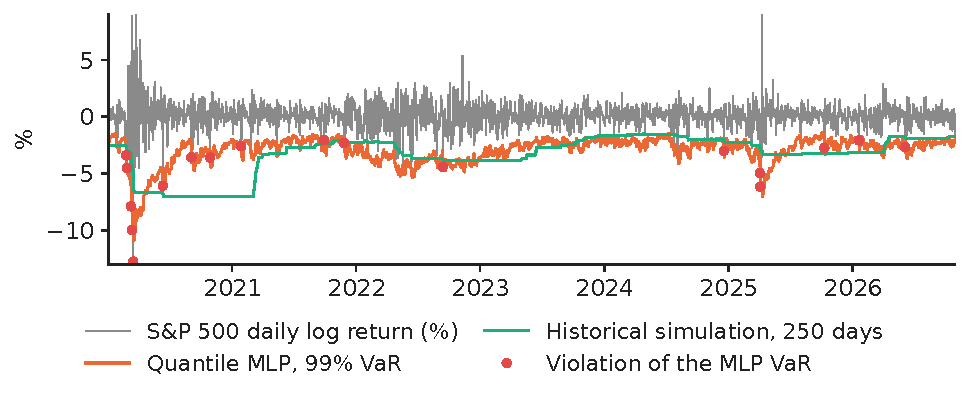
\includegraphics[width=\textwidth,height=0.380\textheight,keepaspectratio]{charts/en/var_backtest.pdf}\end{center}\vspace{-3mm}
\chartsource{Source: Yahoo Finance, daily quotes. Data: 3 Jan 2020 to 30 Oct 2026, trading days (test period).}
\vspace{0.5mm}
\begin{itemize}\setlength{\itemsep}{0pt}
  \item Violations over 1\,716 days (expected 17.2): MLP 18, historical simulation 31, EWMA 41
    \begin{itemize}\setlength{\itemsep}{0pt}
      \item Mean VaR 2.96\,\%, 3.28\,\%, 2.52\,\%.
    \end{itemize}
\end{itemize}
\par\vfill\manager{a VaR that reacts to volatility within days avoids the clusters of breaches of historical simulation.}\par\vspace{0.5mm}
\par\vfill\noindent{\scriptsize\color{FooterGray}(own computation)}\hfill\qlink{NN\_L2\_var\_backtest}{Quantlets/L2/NN_L2_var_backtest}\par\vspace{0.5mm}
\end{frame}

\begin{frame}{The Kupiec test accepts the MLP and rejects both benchmarks}
\small
\intuition{if the VaR is right, the number of breaches is binomial with probability $\tau$; test the observed rate against it.}
\[ \mathrm{LR}_{\mathrm{POF}}=-2\ln\frac{(1-\tau)^{n-x}\tau^{x}}{(1-\hat\pi)^{n-x}\hat\pi^{x}}\ \sim\ \chi^2_1,\quad \hat\pi=\frac xn,\ n\ \text{days},\ x\ \text{violations} \]
{\footnotesize\renewcommand{\arraystretch}{1.05}\setlength{\tabcolsep}{4pt}
\begin{tabular}{@{}lrrrrr@{}}\toprule
Model & Violations & Rate (\%) & $\mathrm{LR}_{\mathrm{POF}}$ & $p$ & Pinball loss \\ \midrule
Quantile MLP (5 seeds) & 18 & 1.05 & 0.04 & 0.840 & 0.0420 \\
Historical simulation, 250 days & 31 & 1.81 & 9.10 & 0.003 & 0.0577 \\
EWMA, $\lambda=0.94$ & 41 & 2.39 & 24.08 & 0.000 & 0.0473 \\
\bottomrule\end{tabular}}
\par\vspace{0.5mm}{\scriptsize \begin{itemize}\setlength{\itemsep}{0pt}
  \item Individual seeds give violation rates between 1.05\,\% and 1.22\,\%; the pinball loss is the proper score for comparing quantile forecasts.
\end{itemize}}
\par\vfill\manager{a regulator looks at the breach count first
    \begin{itemize}\setlength{\itemsep}{0pt}
      \item A risk manager should also compare pinball losses.
    \end{itemize}}\par\vspace{0.5mm}
\par\vfill\noindent{\scriptsize\color{FooterGray}(Kupiec, 1995)}\hfill\tryit{notebook \S8}\par\vspace{0.5mm}
\end{frame}

\begin{frame}{Training hardware: a laptop GPU is ten times faster than its main processor on a large MLP}
\small
\intuition{training is matrix multiplication; a graphics processing unit (GPU) runs thousands of them in parallel.}
\begin{itemize}\setlength{\itemsep}{4pt}
  \item Measured on this course's laptop (arm64, Darwin): one Adam step of an MLP 2048-2048 (4\,216\,833 parameters) on a batch of 2,048 real California rows takes 333.6 ms on the central processing unit (CPU, 4 threads) and 32.5 ms on the GPU through Metal Performance Shaders (MPS): 10.3 times faster.
  \item The small tabular nets of Lectures 1--3 train faster on one CPU thread: copying tiny batches to the GPU costs more than it saves.
  \item On Google Colab the same code runs on an NVIDIA GPU with \texttt{device='cuda'}
    \begin{itemize}\setlength{\itemsep}{0pt}
      \item Set it once and move model and data with \texttt{.to(device)}.
    \end{itemize}
\end{itemize}
\par\vfill\manager{measure before you buy: for tabular models a CPU is enough, for images and text a GPU is not optional.}\par\vspace{0.5mm}
\par\vfill\noindent{\scriptsize\color{FooterGray}(own computation)}\hfill\tryit{notebook \S9}\par\vspace{0.5mm}
\end{frame}

\begin{frame}{A default training procedure}
\small
\begin{columns}[T,onlytextwidth]
\begin{column}{0.49\textwidth}
\begin{block}{Before training}
\begin{itemize}\setlength{\itemsep}{2pt}
  \item Standardise inputs on the training set
    \begin{itemize}\setlength{\itemsep}{0pt}
      \item Split in time order when time matters.
    \end{itemize}
  \item ReLU layers with He initialisation
    \begin{itemize}\setlength{\itemsep}{0pt}
      \item Output and loss from the target (MSE, cross-entropy, pinball).
    \end{itemize}
  \item Overfit one small batch first: if the loss does not go to zero, there is a bug.
\end{itemize}
\end{block}
\end{column}
\begin{column}{0.49\textwidth}
\begin{exampleblock}{During training}
\begin{itemize}\setlength{\itemsep}{2pt}
  \item AdamW, $\eta$ on a log grid around $10^{-3}$, batch 64--256, cosine schedule.
  \item Watch training and validation loss every epoch
    \begin{itemize}\setlength{\itemsep}{0pt}
      \item Keep the best validation weights (Lecture 3).
    \end{itemize}
  \item Repeat with at least 3--5 seeds before claiming a gain.
\end{itemize}
\end{exampleblock}
\end{column}
\end{columns}
\par\vfill\manager{write the recipe into the model documentation: it is what makes a result reproducible.}\par\vspace{0.5mm}
\end{frame}


\section{Wrap-up}

\begin{frame}{Key takeaways}
\small
\begin{itemize}\setlength{\itemsep}{4pt}
  \item Training is gradient descent on the empirical risk
    \begin{itemize}\setlength{\itemsep}{0pt}
      \item Conditioning and the learning rate set its speed and stability.
    \end{itemize}
  \item Backpropagation is the chain rule in reverse: all gradients for about the cost of one more forward pass
    \begin{itemize}\setlength{\itemsep}{0pt}
      \item Check custom code numerically.
    \end{itemize}
  \item Saturating activations and bad initial scales make gradients vanish
    \begin{itemize}\setlength{\itemsep}{0pt}
      \item ReLU with He initialisation keeps them alive.
    \end{itemize}
  \item Momentum and adaptive steps (Adam, AdamW) reach good solutions faster and more reliably across seeds
    \begin{itemize}\setlength{\itemsep}{0pt}
      \item Schedules lower the final error.
    \end{itemize}
  \item The loss defines the product: with the pinball loss, an MLP gives a 99\,\% VaR that passes the Kupiec test (18 breaches, expected 17.2).
\end{itemize}
\end{frame}

\begin{frame}{Key equations}
\small
\begin{columns}[T,onlytextwidth]
\begin{column}{0.49\textwidth}
\[ \btheta_{t+1}=\btheta_t-\eta\,\mathbf g_t,\quad 0<\eta<2/\lambda_{\max} \]
\[ \boldsymbol\delta^{(l)}=(\mW^{(l+1)\top}\boldsymbol\delta^{(l+1)})\odot a'(\vz^{(l)}) \]
\[ \partial\ell/\partial\mW^{(l)}=\boldsymbol\delta^{(l)}\vh^{(l-1)\top} \]
\[ \Var(W)=2/n_{\text{in}}\ \ (\text{He}) \]
\end{column}
\begin{column}{0.49\textwidth}
\[ \mathbf v_{t+1}=\beta\mathbf v_t+\mathbf g_t \]
\[ \theta_{t+1}=\theta_t-\eta\,\hat m_t/(\sqrt{\hat v_t}+\epsilon) \]
\[ \eta_t=\tfrac{\eta_0}{2}(1+\cos\pi t/T) \]
\[ \rho_\tau(u)=u(\tau-\mathbb 1\{u<0\}) \]
\end{column}
\end{columns}
\end{frame}

\begin{frame}{Research from our group: risk forecasts without gradient training}
\small
\begin{itemize}\setlength{\itemsep}{5pt}
  \item \textbf{Risk from language models} (Pele et al., 2026): value at risk and expected shortfall (ES) are obtained by prompting general-purpose large language models (LLM) with the return history (LLM-VaR, LLM-ES), without any task-specific gradient training --- Lecture 12.
  \item \textbf{Foundation models for tail risk} (Jheng, Tak, Găman, Mazurencu-Marinescu-Pele \& Pele, 2026): pretrained time-series foundation models forecast VaR and ES zero-shot, and conformal calibration corrects their coverage, in Central and Eastern European markets --- Lecture 13.
  \item \textbf{How they relate to this lecture}: the same backtests (violation counts, Kupiec test, pinball loss) compare our gradient-trained quantile MLP with these pretrained models.
\end{itemize}
\par\vspace{0.5mm}{\scriptsize \begin{itemize}\setlength{\itemsep}{0pt}
  \item Findings as stated in the papers; numbers on the other slides come from our own computations.
\end{itemize}}
\end{frame}

\begin{frame}{Further reading and resources}
\small
\begin{columns}[T,onlytextwidth]
\begin{column}{0.52\textwidth}
\begin{itemize}\setlength{\itemsep}{4pt}
  \item \textbf{Bishop \& Bishop (2024)}, chapters 7--8: gradient descent and backpropagation: \href{https://www.bishopbook.com}{bishopbook.com}.
  \item \textbf{Dive into Deep Learning}, chapter 12 (optimisation algorithms): \href{https://d2l.ai/chapter_optimization}{d2l.ai}.
  \item \textbf{A. Karpathy, micrograd}: backpropagation in 100 lines: \href{https://github.com/karpathy/micrograd}{github.com/karpathy/micrograd}.
\end{itemize}
\end{column}
\begin{column}{0.45\textwidth}
\begin{itemize}\setlength{\itemsep}{4pt}
  \item \textbf{PyTorch autograd tutorial}: \href{https://pytorch.org/tutorials/beginner/blitz/autograd_tutorial.html}{pytorch.org/tutorials}.
  \item \textbf{This course}: code, data, notebooks, Quantlets --- \href{https://github.com/danpele/NEURAL_BIZ}{github.com/danpele/NEURAL\_BIZ}.
  \item \textbf{Original papers}: Kingma \& Ba (2015), Loshchilov \& Hutter (2019).
\end{itemize}
\end{column}
\end{columns}
\end{frame}

\begin{frame}{Quiz 1: the stable step size}
\small
\begin{itemize}
  \item The raw-income regression has Hessian eigenvalues 0.372 and 38.81.
    \begin{itemize}\setlength{\itemsep}{0pt}
      \item Up to which learning rate does gradient descent converge?
    \end{itemize}
\end{itemize}
\vspace{2mm}
\begin{exampleblock}{Answer}
\begin{itemize}
  \item $\eta<2/\lambda_{\max}=$ 0.0515
    \begin{itemize}\setlength{\itemsep}{0pt}
      \item With $\kappa=$ 104.3 the flat direction contracts very slowly: standardise or use momentum.
    \end{itemize}
\end{itemize}
\end{exampleblock}
\end{frame}

\begin{frame}{Quiz 2: a dead ReLU}
\small
\begin{itemize}
  \item In the hand-computed example, why is $\partial\ell/\partial W^{(1)}_{2j}=0$ for both inputs?
\end{itemize}
\vspace{2mm}
\begin{exampleblock}{Answer}
\begin{itemize}
  \item Unit 2 has $z_2=$ \ensuremath{-}0.093 $<0$, so $\mathbb 1\{z_2>0\}=0$ and $\delta^{(1)}_2=0$: a ReLU that is off passes no gradient.
\end{itemize}
\end{exampleblock}
\end{frame}

\begin{frame}{Quiz 3: vanishing gradients}
\small
\begin{itemize}
  \item Why does a 10-layer sigmoid network learn its first layers so slowly?
\end{itemize}
\vspace{2mm}
\begin{exampleblock}{Answer}
\begin{itemize}
  \item The backward signal is multiplied by $\sigma'\le0.25$ at each layer
    \begin{itemize}\setlength{\itemsep}{0pt}
      \item On our batch the first-layer gradient norm is $8.5\times10^{-7}$.
    \end{itemize}
\end{itemize}
\end{exampleblock}
\end{frame}

\begin{frame}{Quiz 4: Adam's bias correction}
\small
\begin{itemize}
  \item At step $t=1$, with $m_0=0$ and $\beta_1=0.9$, what are $m_1$ and $\hat m_1$?
\end{itemize}
\vspace{2mm}
\begin{exampleblock}{Answer}
\begin{itemize}
  \item $m_1=0.1\,g_1$, biased towards zero
    \begin{itemize}\setlength{\itemsep}{0pt}
      \item $\hat m_1=m_1/(1-0.9)=g_1$, the correction removes the bias.
    \end{itemize}
\end{itemize}
\end{exampleblock}
\end{frame}

\begin{frame}{Quiz 5: backtesting a VaR}
\small
\begin{itemize}
  \item Over 1\,716 test days, how many breaches of a correct 99\,\% VaR do we expect, and which model passes the Kupiec test?
\end{itemize}
\vspace{2mm}
\begin{exampleblock}{Answer}
\begin{itemize}
  \item About 17.2
    \begin{itemize}\setlength{\itemsep}{0pt}
      \item The quantile MLP has 18 ($p=$ 0.840), historical simulation 31 ($p=$ 0.003): only the MLP passes.
    \end{itemize}
\end{itemize}
\end{exampleblock}
\end{frame}

\begin{frame}{References (1/2)}
\scriptsize
\begin{itemize}\setlength{\itemsep}{0pt}\scriptsize
\item Baydin, A.\,G., Pearlmutter, B.\,A., Radul, A.\,A.\ \& Siskind, J.\,M.\ (2018). Automatic differentiation in machine learning: a survey. \textit{Journal of Machine Learning Research}, 18(153), 1--43. \href{https://arxiv.org/abs/1502.05767}{arXiv:1502.05767}
\item Bengio, Y., Simard, P.\ \& Frasconi, P.\ (1994). Learning long-term dependencies with gradient descent is difficult. \textit{IEEE Transactions on Neural Networks}, 5(2), 157--166. \href{https://doi.org/10.1109/72.279181}{doi:10.1109/72.279181}
\item Bishop, C.\,M.\ \& Bishop, H.\ (2024). \textit{Deep Learning: Foundations and Concepts}. Springer. \href{https://doi.org/10.1007/978-3-031-45468-4}{doi:10.1007/978-3-031-45468-4}
\item Dal Pozzolo, A., Caelen, O., Johnson, R.\,A.\ \& Bontempi, G.\ (2015). Calibrating probability with undersampling for unbalanced classification. \textit{IEEE Symposium Series on Computational Intelligence}, 159--166. \href{https://doi.org/10.1109/SSCI.2015.33}{doi:10.1109/SSCI.2015.33}
\item Duchi, J., Hazan, E.\ \& Singer, Y.\ (2011). Adaptive subgradient methods for online learning and stochastic optimization. \textit{Journal of Machine Learning Research}, 12, 2121--2159.
\item Glorot, X.\ \& Bengio, Y.\ (2010). Understanding the difficulty of training deep feedforward neural networks. \textit{Proceedings of AISTATS}, PMLR 9, 249--256.
\item He, K., Zhang, X., Ren, S.\ \& Sun, J.\ (2015). Delving deep into rectifiers. \textit{IEEE International Conference on Computer Vision}, 1026--1034. \href{https://doi.org/10.1109/ICCV.2015.123}{doi:10.1109/ICCV.2015.123}
\item Jheng, S.-L., Tak, R., Găman, Ș., Mazurencu-Marinescu-Pele, M.\ \& Pele, D.\,T.\ (2026). Can foundation models manage risk? Zero-shot VaR and ES forecasting with conformal calibration in CEE markets. \textit{Economic Computation and Economic Cybernetics Studies and Research}, 60(2), 267--290. \href{https://doi.org/10.24818/18423264/60.2.26.14}{doi:10.24818/18423264/60.2.26.14}
\item Keskar, N.\,S., Mudigere, D., Nocedal, J., Smelyanskiy, M.\ \& Tang, P.\,T.\,P.\ (2017). On large-batch training for deep learning: Generalization gap and sharp minima. \textit{International Conference on Learning Representations}. \href{https://arxiv.org/abs/1609.04836}{arXiv:1609.04836}
\item Kingma, D.\,P.\ \& Ba, J.\ (2015). Adam: A method for stochastic optimization. \textit{International Conference on Learning Representations}. \href{https://arxiv.org/abs/1412.6980}{arXiv:1412.6980}
\item Koenker, R.\ \& Bassett, G.\ (1978). Regression quantiles. \textit{Econometrica}, 46(1), 33--50. \href{https://doi.org/10.2307/1913643}{doi:10.2307/1913643}
\end{itemize}
\end{frame}

\begin{frame}{References (2/2)}
\scriptsize
\begin{itemize}\setlength{\itemsep}{0pt}\scriptsize
\item Kupiec, P.\,H.\ (1995). Techniques for verifying the accuracy of risk measurement models. \textit{The Journal of Derivatives}, 3(2), 73--84. \href{https://doi.org/10.3905/jod.1995.407942}{doi:10.3905/jod.1995.407942}
\item Loshchilov, I.\ \& Hutter, F.\ (2017). SGDR: Stochastic gradient descent with warm restarts. \textit{International Conference on Learning Representations}. \href{https://arxiv.org/abs/1608.03983}{arXiv:1608.03983}
\item Loshchilov, I.\ \& Hutter, F.\ (2019). Decoupled weight decay regularization. \textit{International Conference on Learning Representations}. \href{https://arxiv.org/abs/1711.05101}{arXiv:1711.05101}
\item Pace, R.\,K.\ \& Barry, R.\ (1997). Sparse spatial autoregressions. \textit{Statistics \& Probability Letters}, 33(3), 291--297. \href{https://doi.org/10.1016/S0167-7152(96)00140-X}{doi:10.1016/S0167-7152(96)00140-X}
\item Paszke, A.\ et al.\ (2019). PyTorch: An imperative style, high-performance deep learning library. \textit{Advances in Neural Information Processing Systems}, 32. \href{https://arxiv.org/abs/1912.01703}{arXiv:1912.01703}
\item Pele, D.\,T., Bolovăneanu, V., Lin, M.-B., Ren, R., Ginavar, A.\,T., Spilak, B., Andrei, A.-V., Toma, F.-M., Lessmann, S.\ \& Härdle, W.\,K.\ (2026). In the beginning was the Word: LLM-VaR and LLM-ES. \textit{Expert Systems with Applications}, 295, 128676. \href{https://doi.org/10.1016/j.eswa.2025.128676}{doi:10.1016/j.eswa.2025.128676}
\item Polyak, B.\,T.\ (1964). Some methods of speeding up the convergence of iteration methods. \textit{USSR Computational Mathematics and Mathematical Physics}, 4(5), 1--17. \href{https://doi.org/10.1016/0041-5553(64)90137-5}{doi:10.1016/0041-5553(64)90137-5}
\item Robbins, H.\ \& Monro, S.\ (1951). A stochastic approximation method. \textit{The Annals of Mathematical Statistics}, 22(3), 400--407. \href{https://doi.org/10.1214/aoms/1177729586}{doi:10.1214/aoms/1177729586}
\item Rumelhart, D.\,E., Hinton, G.\,E.\ \& Williams, R.\,J.\ (1986). Learning representations by back-propagating errors. \textit{Nature}, 323, 533--536. \href{https://doi.org/10.1038/323533a0}{doi:10.1038/323533a0}
\item Smith, L.\,N.\ \& Topin, N.\ (2019). Super-convergence: Very fast training of neural networks using large learning rates. \textit{Proceedings of SPIE}, 11006. \href{https://arxiv.org/abs/1708.07120}{arXiv:1708.07120}
\item Tieleman, T.\ \& Hinton, G.\ (2012). Lecture 6.5 --- RMSProp: Divide the gradient by a running average of its recent magnitude. \textit{COURSERA: Neural Networks for Machine Learning}.
\end{itemize}
\end{frame}

\appendix

\begin{frame}{Appendix: backpropagation in matrix form for a mini-batch}
\small
\[ \mathbf Z^{(l)}=\mathbf H^{(l-1)}\mW^{(l)\top}+\mathbf 1\vb^{(l)\top},\quad \mathbf H^{(l)}=a(\mathbf Z^{(l)}),\qquad \boldsymbol\Delta^{(l)}=\big(\boldsymbol\Delta^{(l+1)}\mW^{(l+1)}\big)\odot a'(\mathbf Z^{(l)}) \]
\[ \frac{\partial\loss}{\partial\mW^{(l)}}=\frac1B\boldsymbol\Delta^{(l)\top}\mathbf H^{(l-1)},\qquad \frac{\partial\loss}{\partial\vb^{(l)}}=\frac1B\boldsymbol\Delta^{(l)\top}\mathbf 1 \]
\begin{itemize}\setlength{\itemsep}{2pt}
  \item Rows of $\mathbf H$, $\mathbf Z$, $\boldsymbol\Delta$ are the $B$ examples of the batch
    \begin{itemize}\setlength{\itemsep}{0pt}
      \item Every step is a matrix product, which is why graphics processors help.
    \end{itemize}
  \item Cost: forward $\sum_l B\,n_{l-1}n_l$ multiply-adds
    \begin{itemize}\setlength{\itemsep}{0pt}
      \item Backward about twice that.
    \end{itemize}
\end{itemize}
\end{frame}

\begin{frame}{Appendix: why Adam needs a bias correction}
\small
\[ m_t=(1-\beta_1)\sum_{k=1}^{t}\beta_1^{t-k}g_k\ \Rightarrow\ \E[m_t]=\E[g]\,(1-\beta_1)\sum_{k=1}^{t}\beta_1^{t-k}=\E[g]\,(1-\beta_1^t) \]
\begin{itemize}\setlength{\itemsep}{2pt}
  \item If the gradient distribution is stationary, $m_t/(1-\beta_1^t)$ is unbiased for $\E[g]$
    \begin{itemize}\setlength{\itemsep}{0pt}
      \item The same holds for $v_t$ and $\E[g^2]$.
    \end{itemize}
  \item With $\beta_2=0.999$, $v_t$ without correction is 1000 times too small at $t=1$: the first steps would be huge.
\end{itemize}
\par\vfill\noindent{\scriptsize\color{FooterGray}(Kingma \& Ba, 2015)}\par\vspace{0.5mm}
\end{frame}

\begin{frame}{Appendix: the Kupiec likelihood-ratio test}
\small
\begin{itemize}\setlength{\itemsep}{5pt}
  \item Violations $I_t=\mathbb 1\{r_t<-\mathrm{VaR}_t\}$
    \begin{itemize}\setlength{\itemsep}{0pt}
      \item Under a correct model, $I_t\iid\text{Bernoulli}(\tau)$ and $x=\sum I_t\sim\text{Bin}(n,\tau)$.
    \end{itemize}
  \item Likelihood under $H_0$: $(1-\tau)^{n-x}\tau^x$
    \begin{itemize}\setlength{\itemsep}{0pt}
      \item Under the alternative, maximised at $\hat\pi=x/n$.
    \end{itemize}
  \item $\mathrm{LR}=-2\ln(L_0/L_1)\to\chi^2_1$
    \begin{itemize}\setlength{\itemsep}{0pt}
      \item Reject at 5\,\% when $\mathrm{LR}>3.84$.
    \end{itemize}
  \item The test checks only the count
    \begin{itemize}\setlength{\itemsep}{0pt}
      \item Independence of the violations needs Christoffersen's test (Lecture 13).
    \end{itemize}
\end{itemize}
\par\vfill\noindent{\scriptsize\color{FooterGray}(Kupiec, 1995)}\par\vspace{0.5mm}
\end{frame}

\end{document}
